\documentclass[titlepage,a4paper]{article}
\usepackage{a4wide}
\usepackage[colorlinks=true,linkcolor=black,urlcolor=blue,bookmarksopen=true]{hyperref}
\usepackage{bookmark}
\usepackage{fancyhdr}
\usepackage[spanish]{babel}
\usepackage[utf8]{inputenc}
\usepackage[T1]{fontenc}
\usepackage{graphicx}
\usepackage{float}
\usepackage{enumerate}
\usepackage{amsmath}
\usepackage{caption}
\usepackage{subfig}

\DeclareCaptionType{equ}[][]

\pagestyle{fancy} % Encabezado y pie de página
\fancyhf{}
\fancyhead[L]{TP - Grupo }
\fancyhead[R]{Orga. de Datos - FIUBA}
\renewcommand{\headrulewidth}{0.4pt}
\fancyfoot[C]{\thepage}
\renewcommand{\footrulewidth}{0.4pt}

\begin{document}
\begin{titlepage} % Carátula
  \hfill
\includegraphics[width=6cm]{logofiuba.jpg}
    \centering
    \vfill
    \Huge \textbf{Organización de Datos (75.06)}
    \vskip1cm
    \Huge \textbf{Análisis Exploratorio}
    \vskip2cm
    \Large Primer Cuatrimestre 2020\\
    Grupo: \\
    Integrantes:\\
    \vfill
    \begin{tabular}{ | l | l | l | } 
      \hline
      Alumno & Padron & Email \\ \hline
      Kevin Mendoza & 98038 & kmendoza@fi.uba.ar \\ \hline
      Sebastián Agustín Rinaldi & 94290 & srinaldi@fi.uba.ar \\ \hline
      Francisco Xavier Gauna & 100563 & fgauna@fi.uba.ar \\ \hline
      Joaquin Parodi & 100752 & jparodi@fi.uba.ar \\ \hline
    \end{tabular}
    \vfill
    \vfill
    Link del Github:\\\textcolor{black}{\underline{\url{https://github.com/FranciscoGauna/TP1-Datos}}}
\end{titlepage}
\tableofcontents % Índice general
\newpage


\section{\Large Introducción}
{\Large 
En el presente informe nos proponemos analizar los datos provistos por el set de datos sobre tweets que se puede descargar desde \textcolor{blue}{\underline{\url{https://www.kaggle.com/c/nlp-getting-started}}} .\\
El objetivo principal es poder ver que información interesante podemos descubrir sobre estos tweets, ya sea que esa información que esté relacionada con la veracidad de los mismos o no. Para poder llevar a cabo esto, que es un informe sobre el análisis exploratorio de los datos, nos basaremos en un proceso iterativo de preguntas y respuestas.
\par}
\section{\Large Información de los datos}\label{sec:infoDatos}
{\Large
Con 7613 registros de 5 atributos cada uno, tenemos registros con valores nulos.\\
Los atributos son los siguientes:
\begin{itemize}
    \item id: Identificador del tweet es único.
    \item text: El texto del tweet.
    \item location: La ubicación desde donde fue enviado.
    \item keyword: La palabra clave para el tweet
    \item target: Indica si un tweet habla de un desastre real(1) o no(0)
\end{itemize}
En el presente trabajo si decimos que un tweet es veraz, nos estaremos refiriendo a que se refiere a un desastre real. En caso contrario, nos referiremos a que no es un desastre real.
\par}
\subsection{\Large Limpieza de datos}
{\Large Antes de comenzar a analizar los datos tenemos que ver si los registros que tenemos en el set de datos están completos. Una de las cosas a tener en cuenta es ver la cantidad de valores nulos que tiene el set.
\par}
\begin{figure}[H]
 \centering
 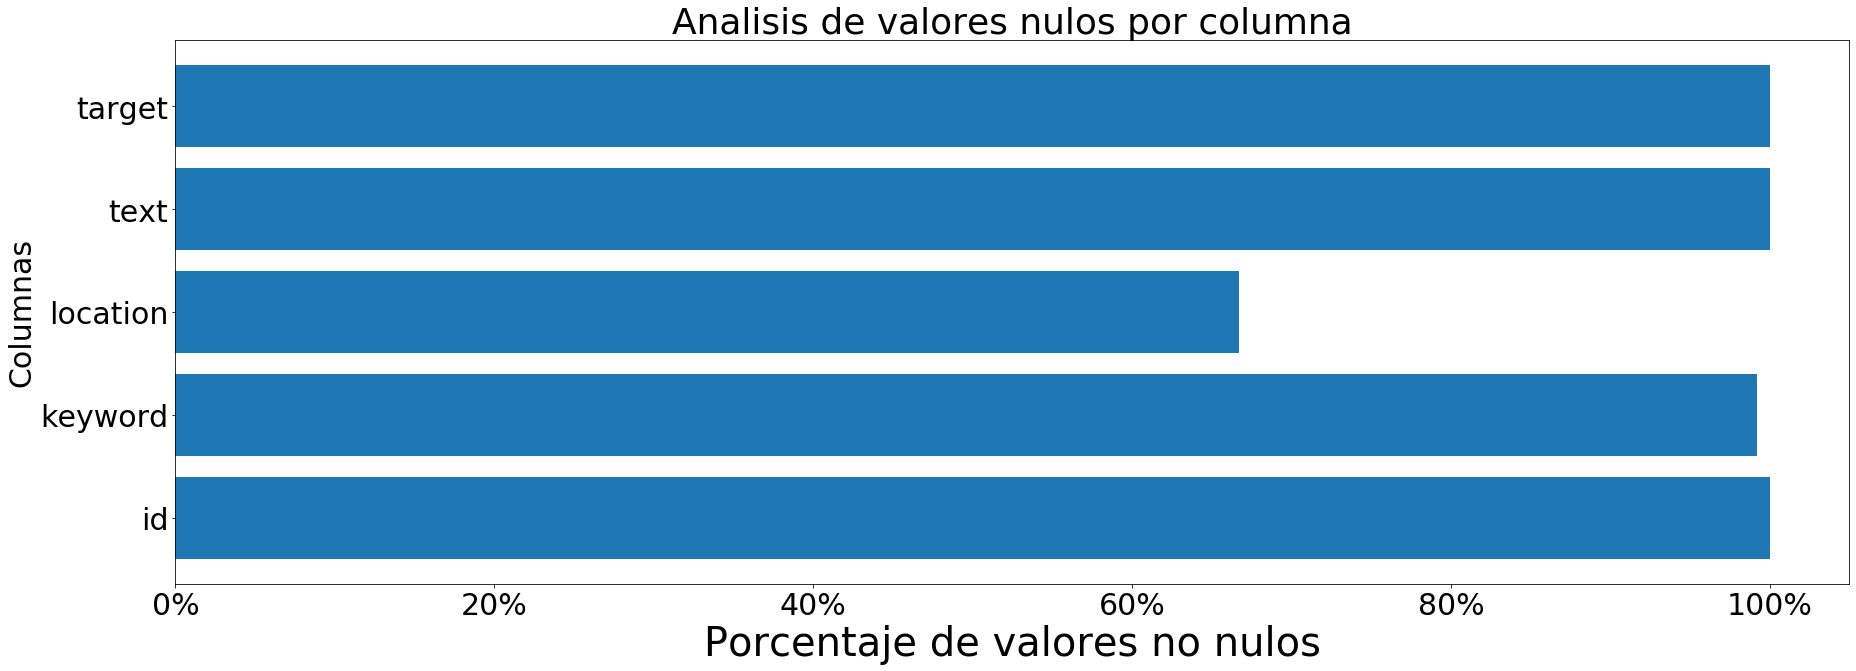
\includegraphics[width=0.8\textwidth, height=0.8\textheight, keepaspectratio]{graficos/porcentajevaloresnonuloscolumnas.png}
\end{figure}
{\Large Lo que se observa es que solo la columna \textbf{location} tiene un faltante de datos importante, por lo que a la hora de hacer análisis relacionados con los valores de esta columna, va a haber que tener en cuenta este dato. Por otro lado se puede ver que la en la columna \textbf{keyword} a pesar de no ser todos valores no nulos, el porcentaje de los nulos es muy muy bajo, por lo que según el análisis que se quiera hacer se determinará que hacer con esos registros.
\par}
{\Large
Justamente como algunos datos no nos llegaron completos, para poder subsanar esto tenemos diferentes métodos que podría ser los siguientes:
\begin{itemize}
    \item Reemplazar el valor nulo por un cero o el valor medio de los datos.
    \item Eliminar la fila, columna donde se encuentra este dato.
\end{itemize}
Los métodos mencionados no son los únicos, pero son los que se utilizaran en este trabajo practico.
\par}
\newpage
\section{\Large Análisis del Texto}
\subsection{\Large Largo del tweet según su veracidad}
{\Large
\begin{figure}[H]
 \centering
 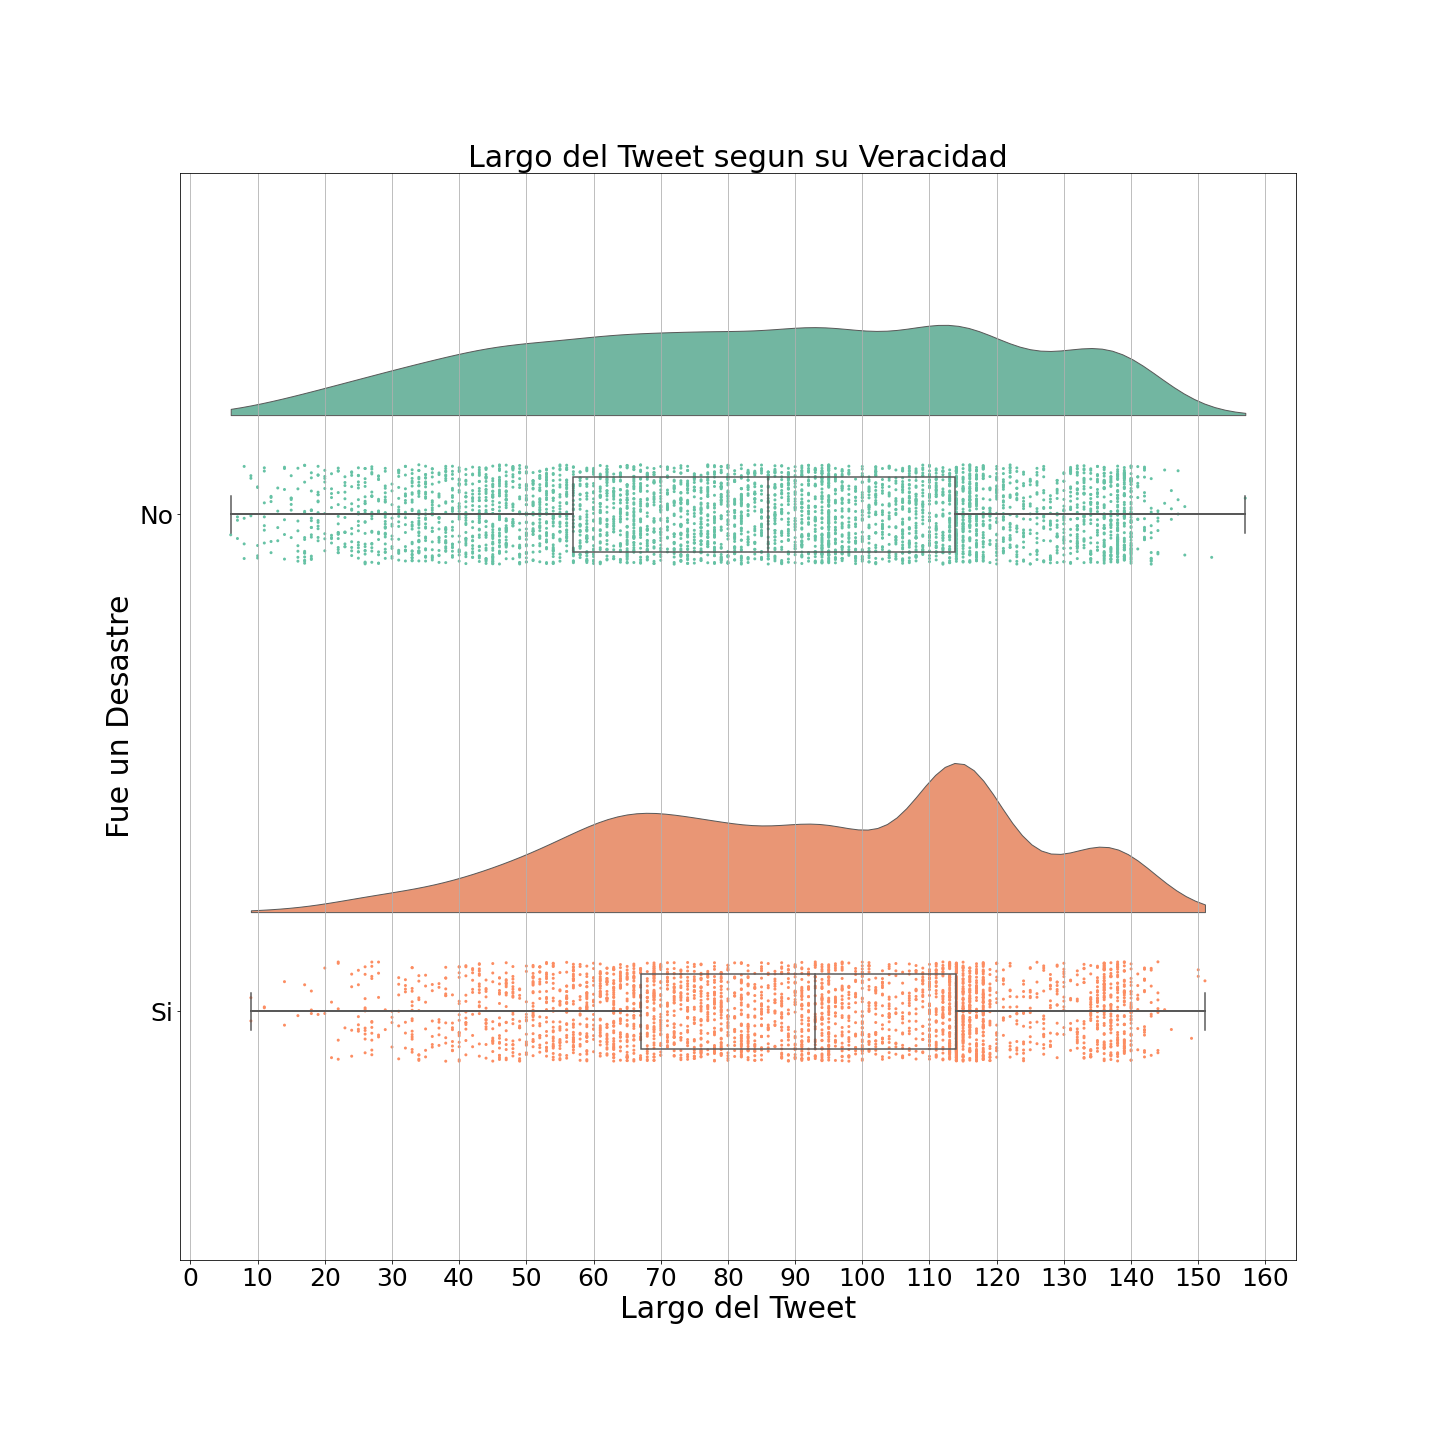
\includegraphics[width=0.8\textwidth, height=0.8\textheight, keepaspectratio]{graficos/largo_tweet_veracidad_0.png}
\end{figure}
Observando el gráfico, los tweets que son desastre presentan una mayor longitud pero no parece ser una diferencia lo suficientemente significativa.
\par}
\subsection{\Large Idiomas de los tweets}
{\Large 
Antes de empezar a analizar el texto de los tweets, nos gustaría saber cuantos tweets por idioma hay, si hay alguno que predomine, etc...
\par}
{\Large
\begin{figure}[H]
 \centering
 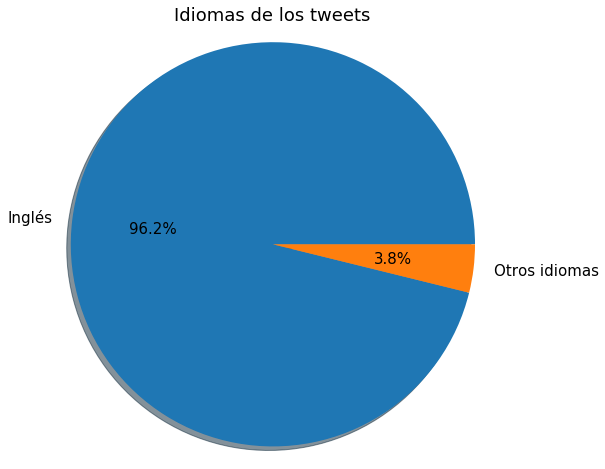
\includegraphics[width=0.7\textwidth, height=0.7\textheight, keepaspectratio]{graficos/idiomasdelostweets.png}
\end{figure}
{\Large 
% Como se puede ver, mas del 96\% de los tweets están en inglés, por lo que algunos de los análisis que hagamos posteriormente sobre las palabras, van a ser tenidos en cuenta pensando en que la mayoría de ellos pertenecen a un solo idioma
\par}
\par}
\subsection{\Large Cantidad de tweets que utilizan hashtags}
{\Large
\begin{figure}[H]
 \centering
 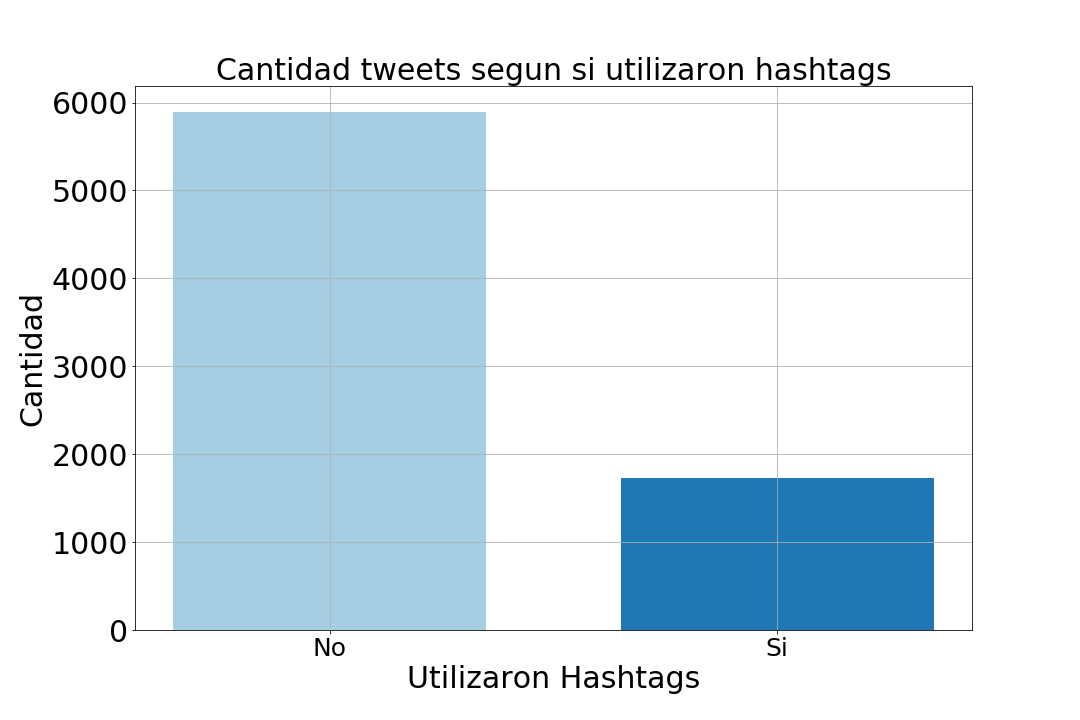
\includegraphics[width=0.8\textwidth, height=0.8\textheight, keepaspectratio]{graficos/cantidad_tweets_utilizaron_hashtags_0.png}
\end{figure}
\begin{figure}[H]
 \centering
 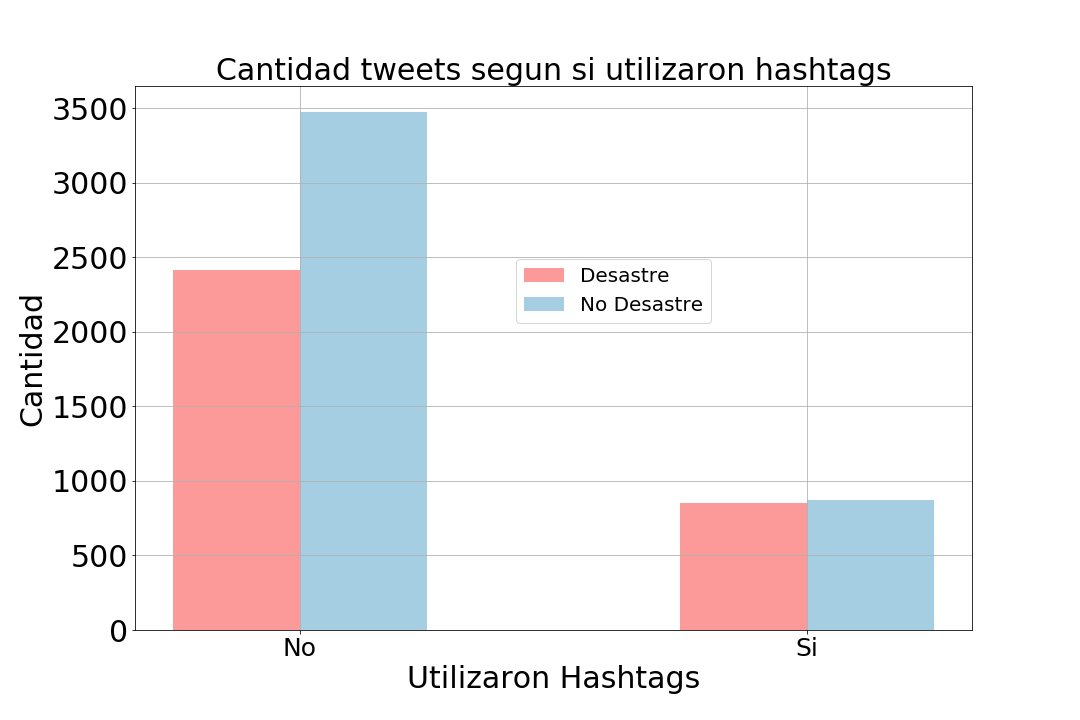
\includegraphics[width=0.8\textwidth, height=0.8\textheight, keepaspectratio]{graficos/cantidad_tweets_utilizaron_hashtags_1.png}
\end{figure}
Sabemos que los hashtags se usan para indexar palabras claves que clasifican los contenidos publicados. Esto permite que haya mayor interacción  entre el contenido y otros usuarios interesados en el tema. Siguiendo esto mas adelante veremos si en los hashtags tenemos la palabra clave que identifica el desastre.
\par}
\subsection{\Large Distribución de la cantidad de hashtags utilizados en tweets}
{\Large
\begin{figure}[H]
 \centering
 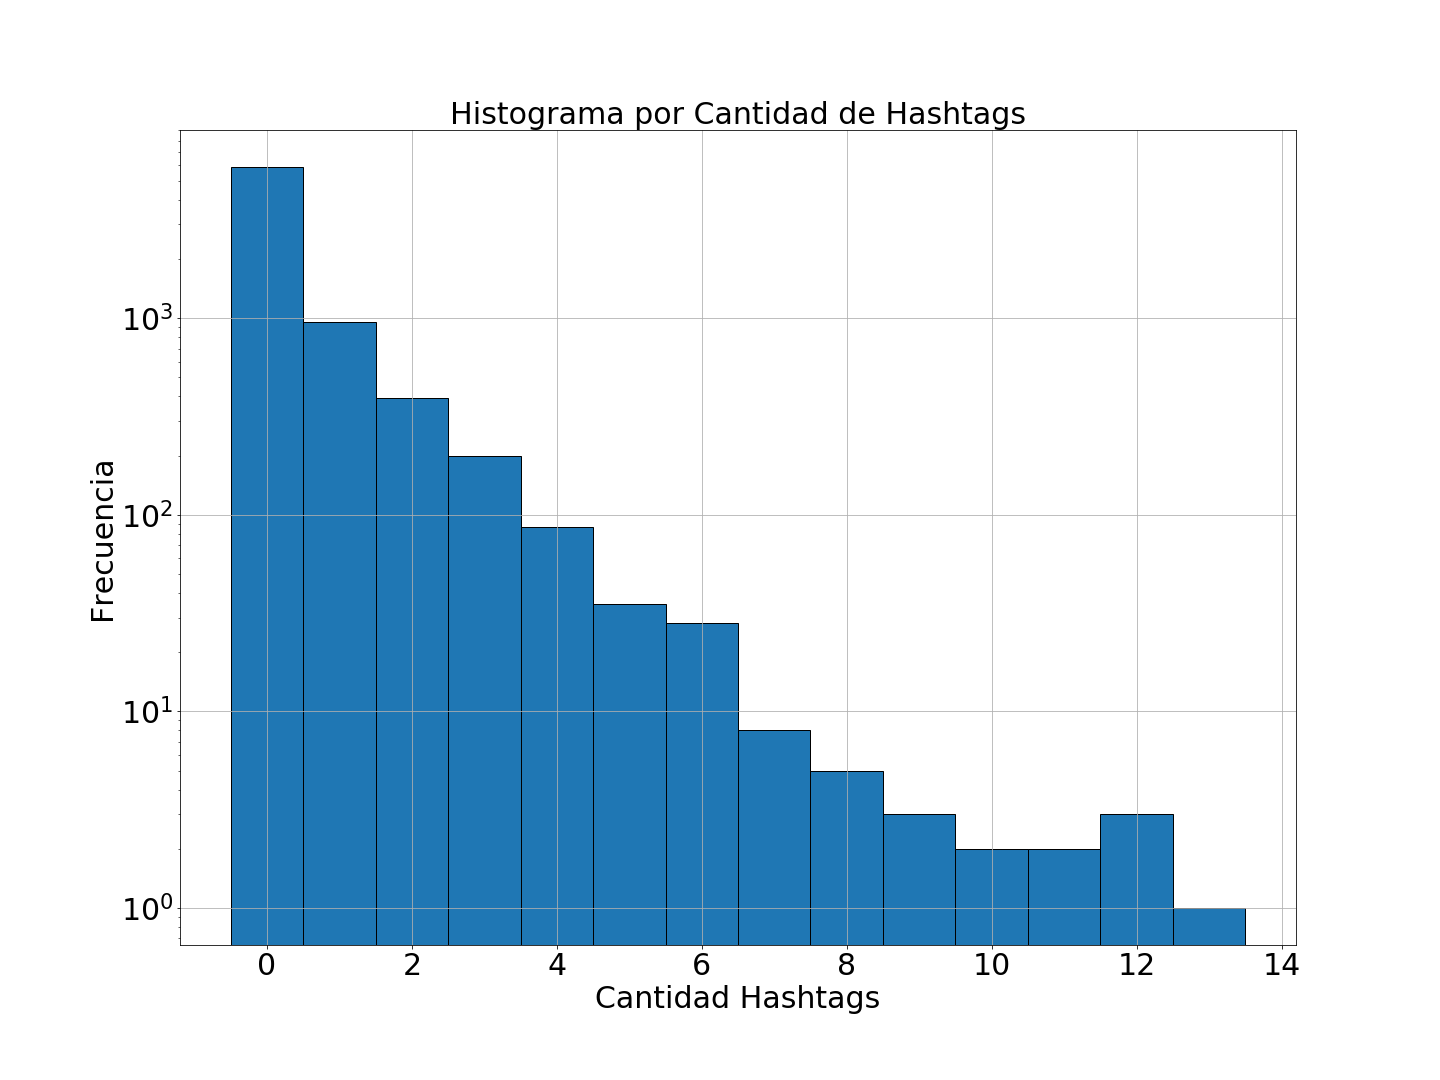
\includegraphics[width=0.8\textwidth, height=0.8\textheight, keepaspectratio]{graficos/histograma_precio_cantidad_hashtags_0.png}
\end{figure}
\begin{figure}[H]
 \centering
 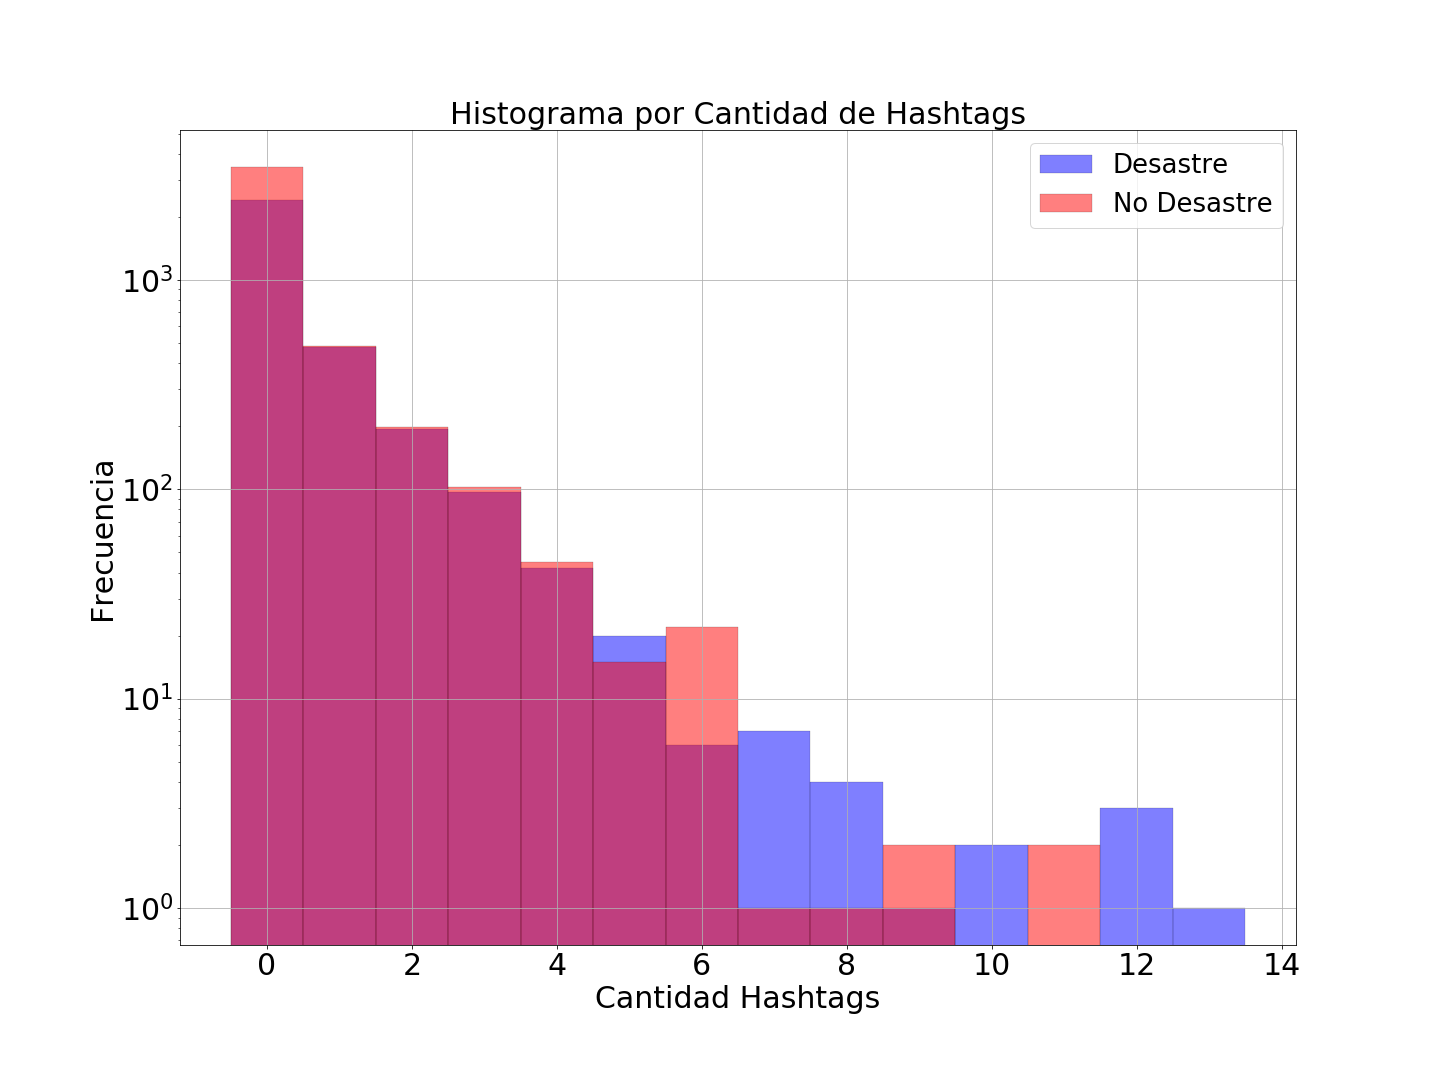
\includegraphics[width=0.8\textwidth, height=0.8\textheight, keepaspectratio]{graficos/histograma_precio_cantidad_hashtags_1.png}
\end{figure}
\par}
\subsection{\Large Hashtags mas populares}
{\Large
\begin{figure}[H]
 \centering
 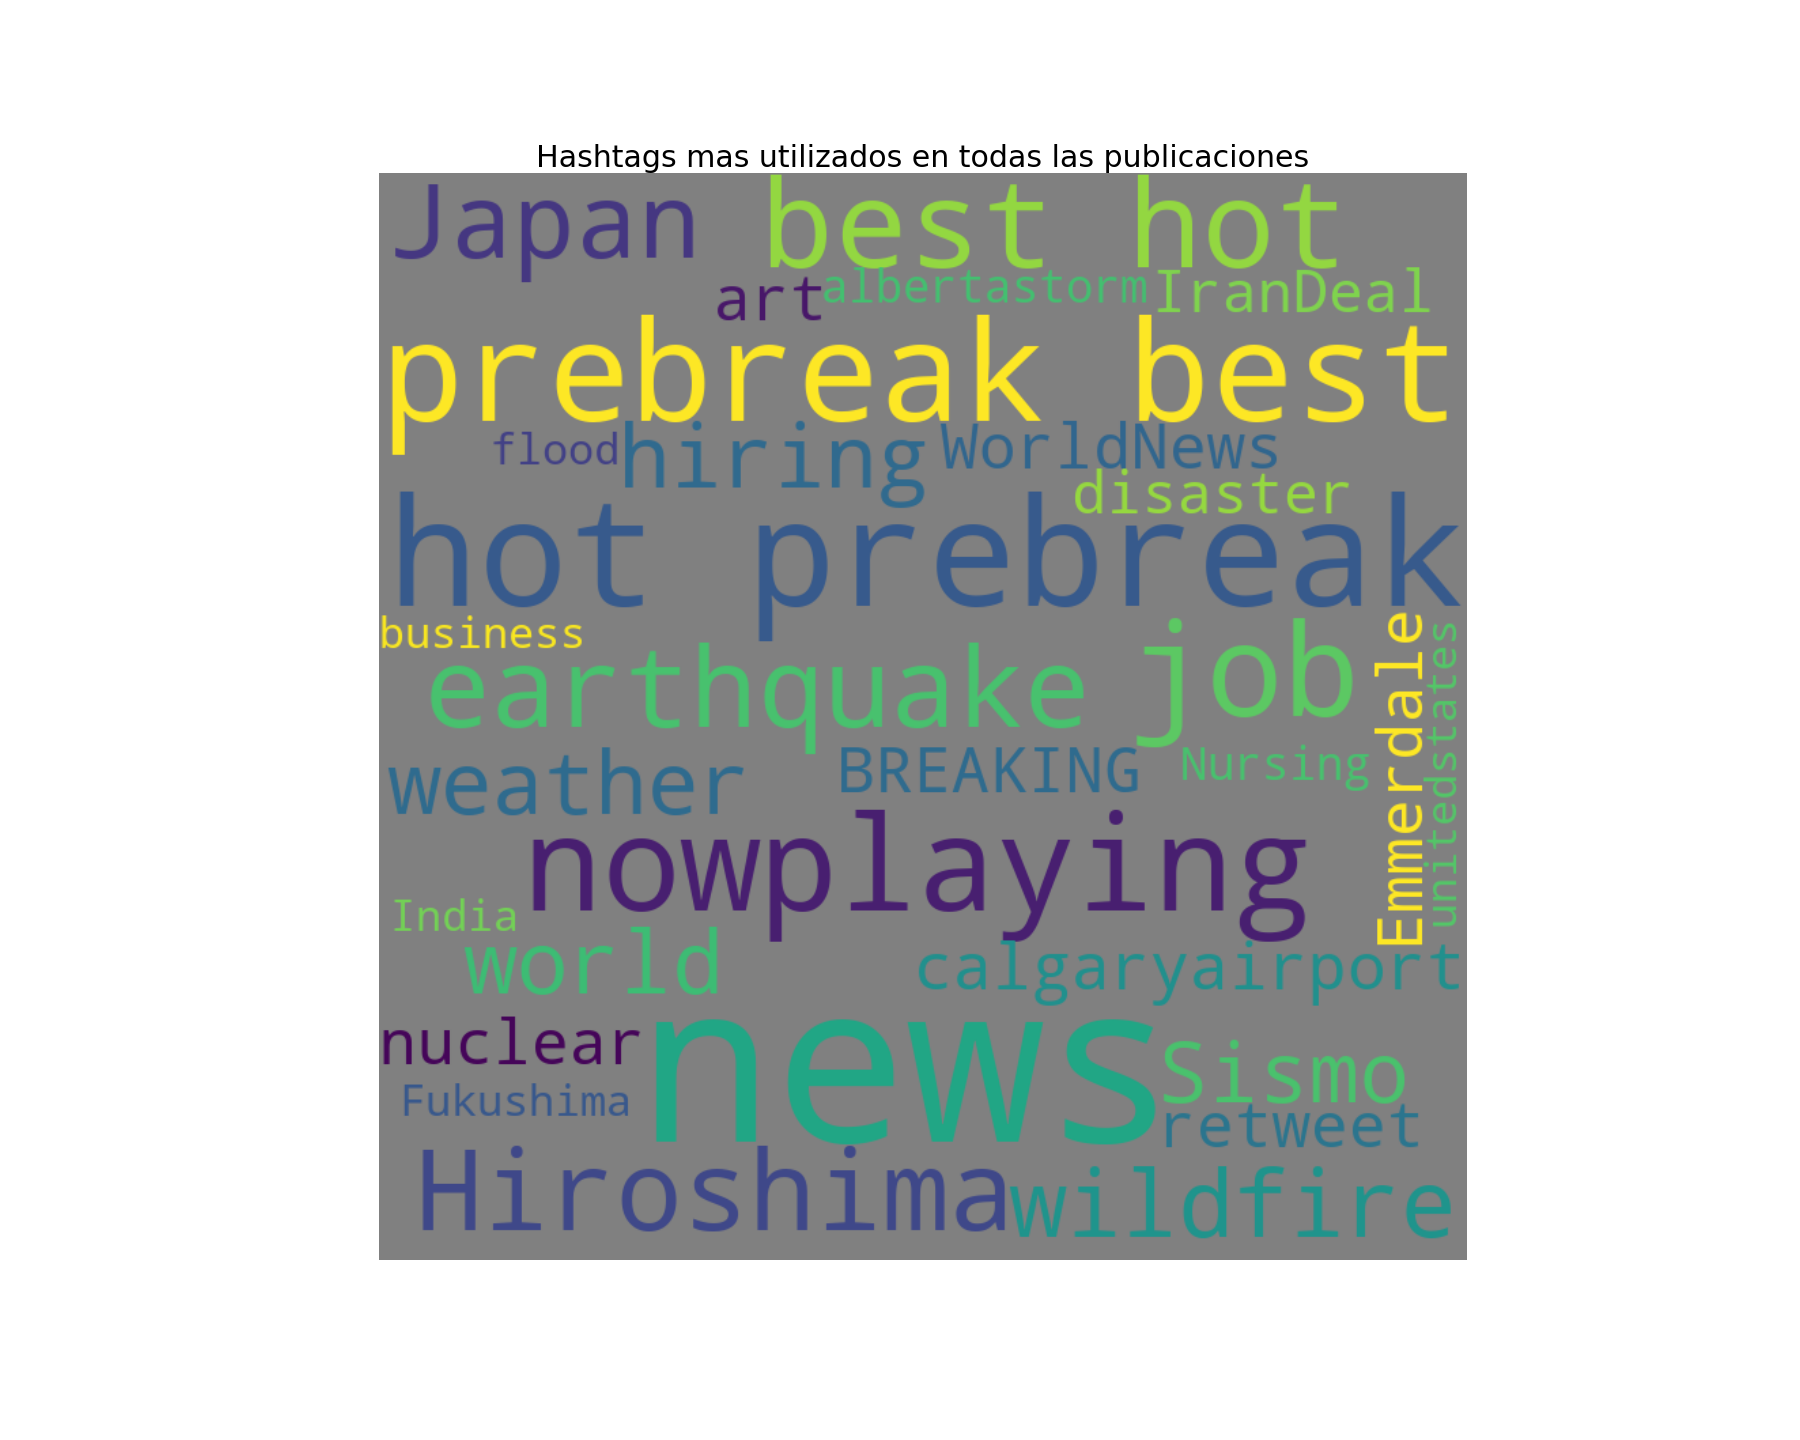
\includegraphics[width=0.85\textwidth, height=0.8\textheight, keepaspectratio]{graficos/analisis_hashtags_0.png}
\end{figure}
\begin{figure}[H]
 \centering
 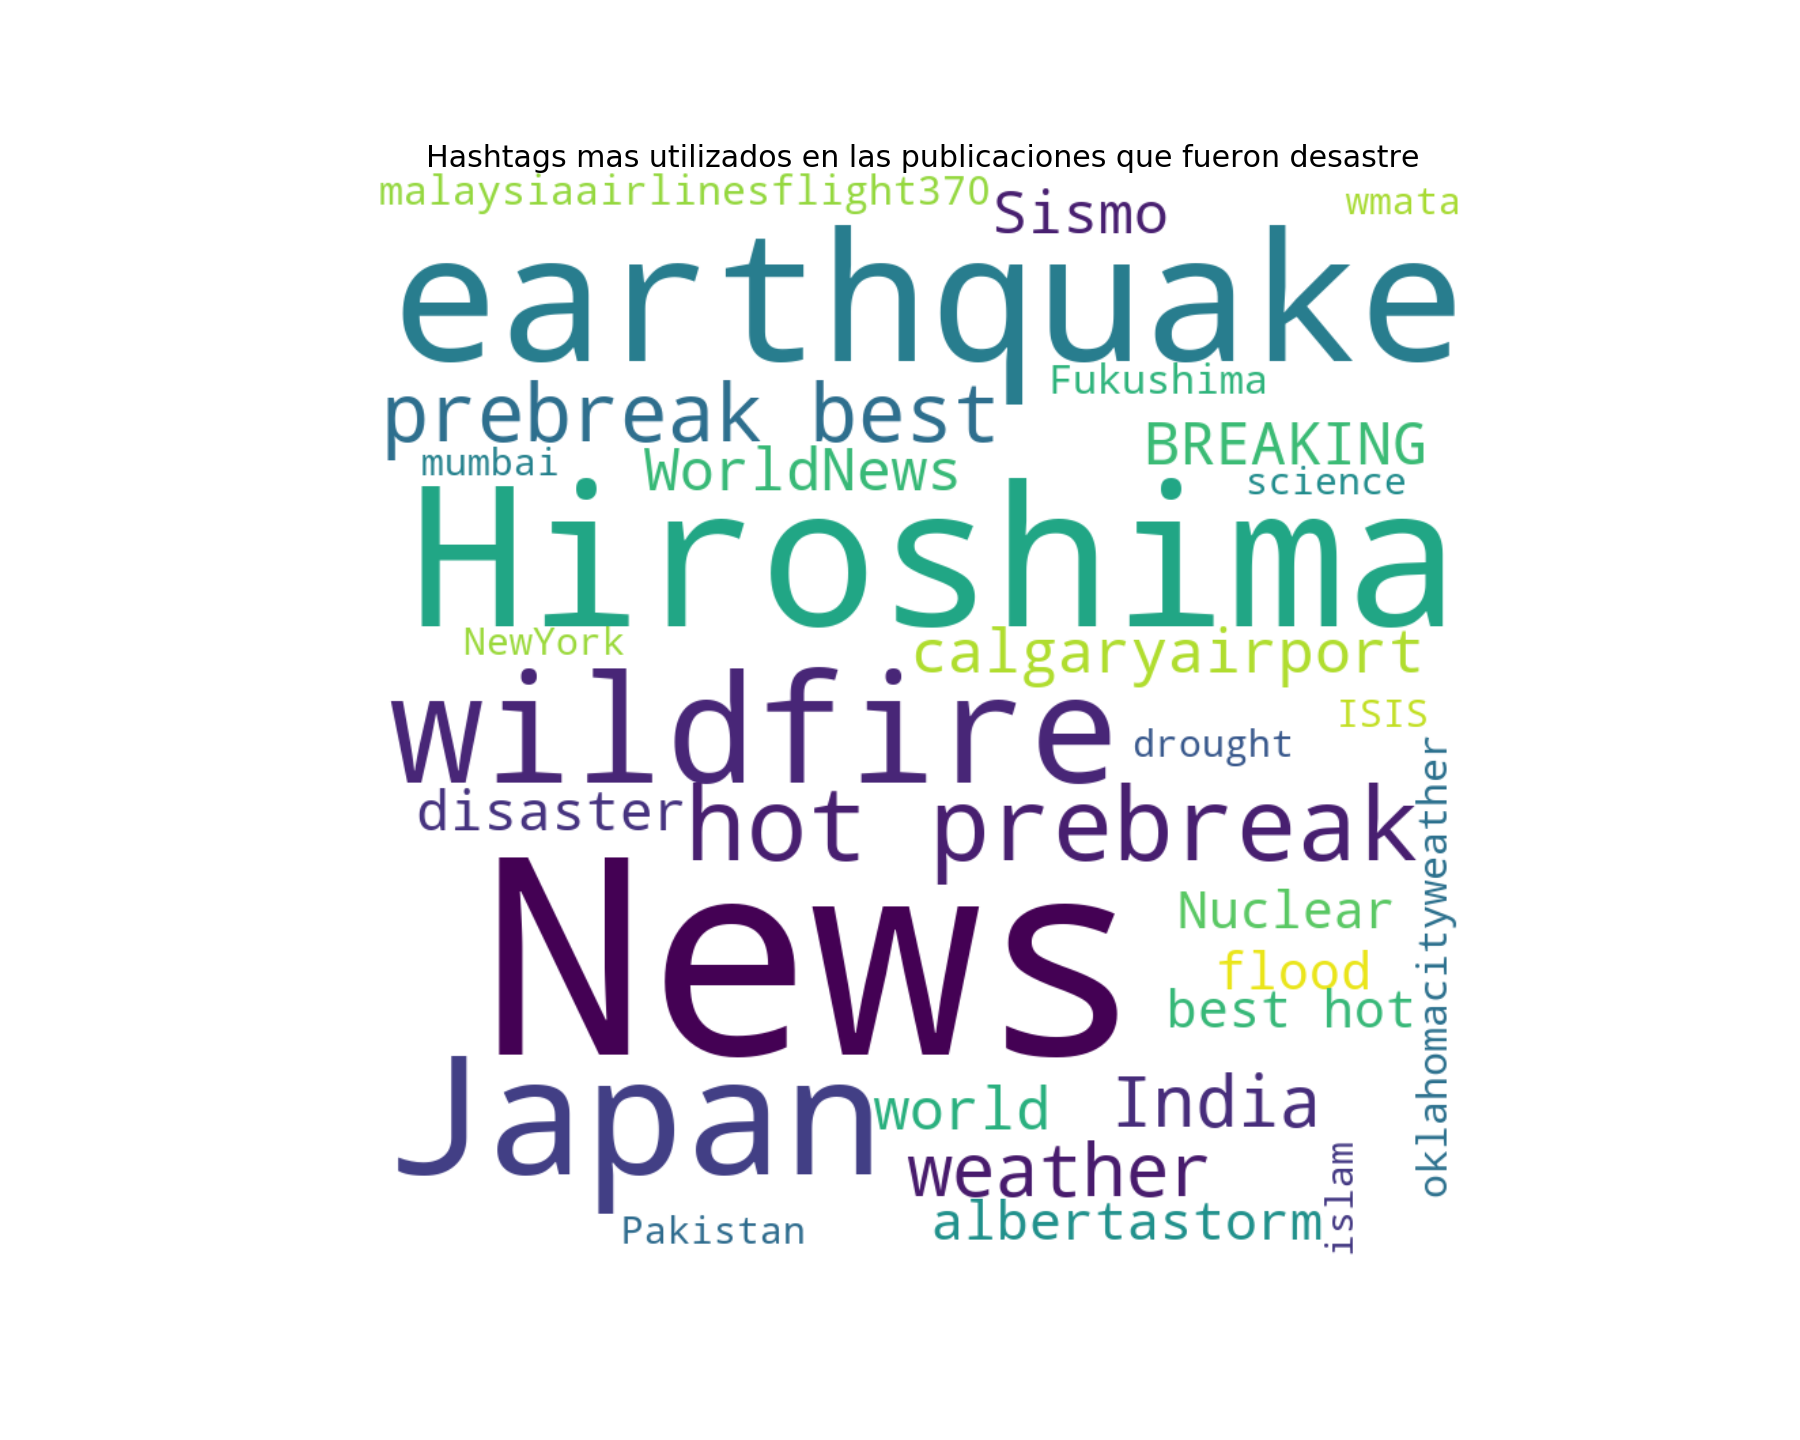
\includegraphics[width=0.85\textwidth, height=0.85\textheight, keepaspectratio]{graficos/analisis_hashtags_1.png}
\end{figure}
\begin{figure}[H]
 \centering
 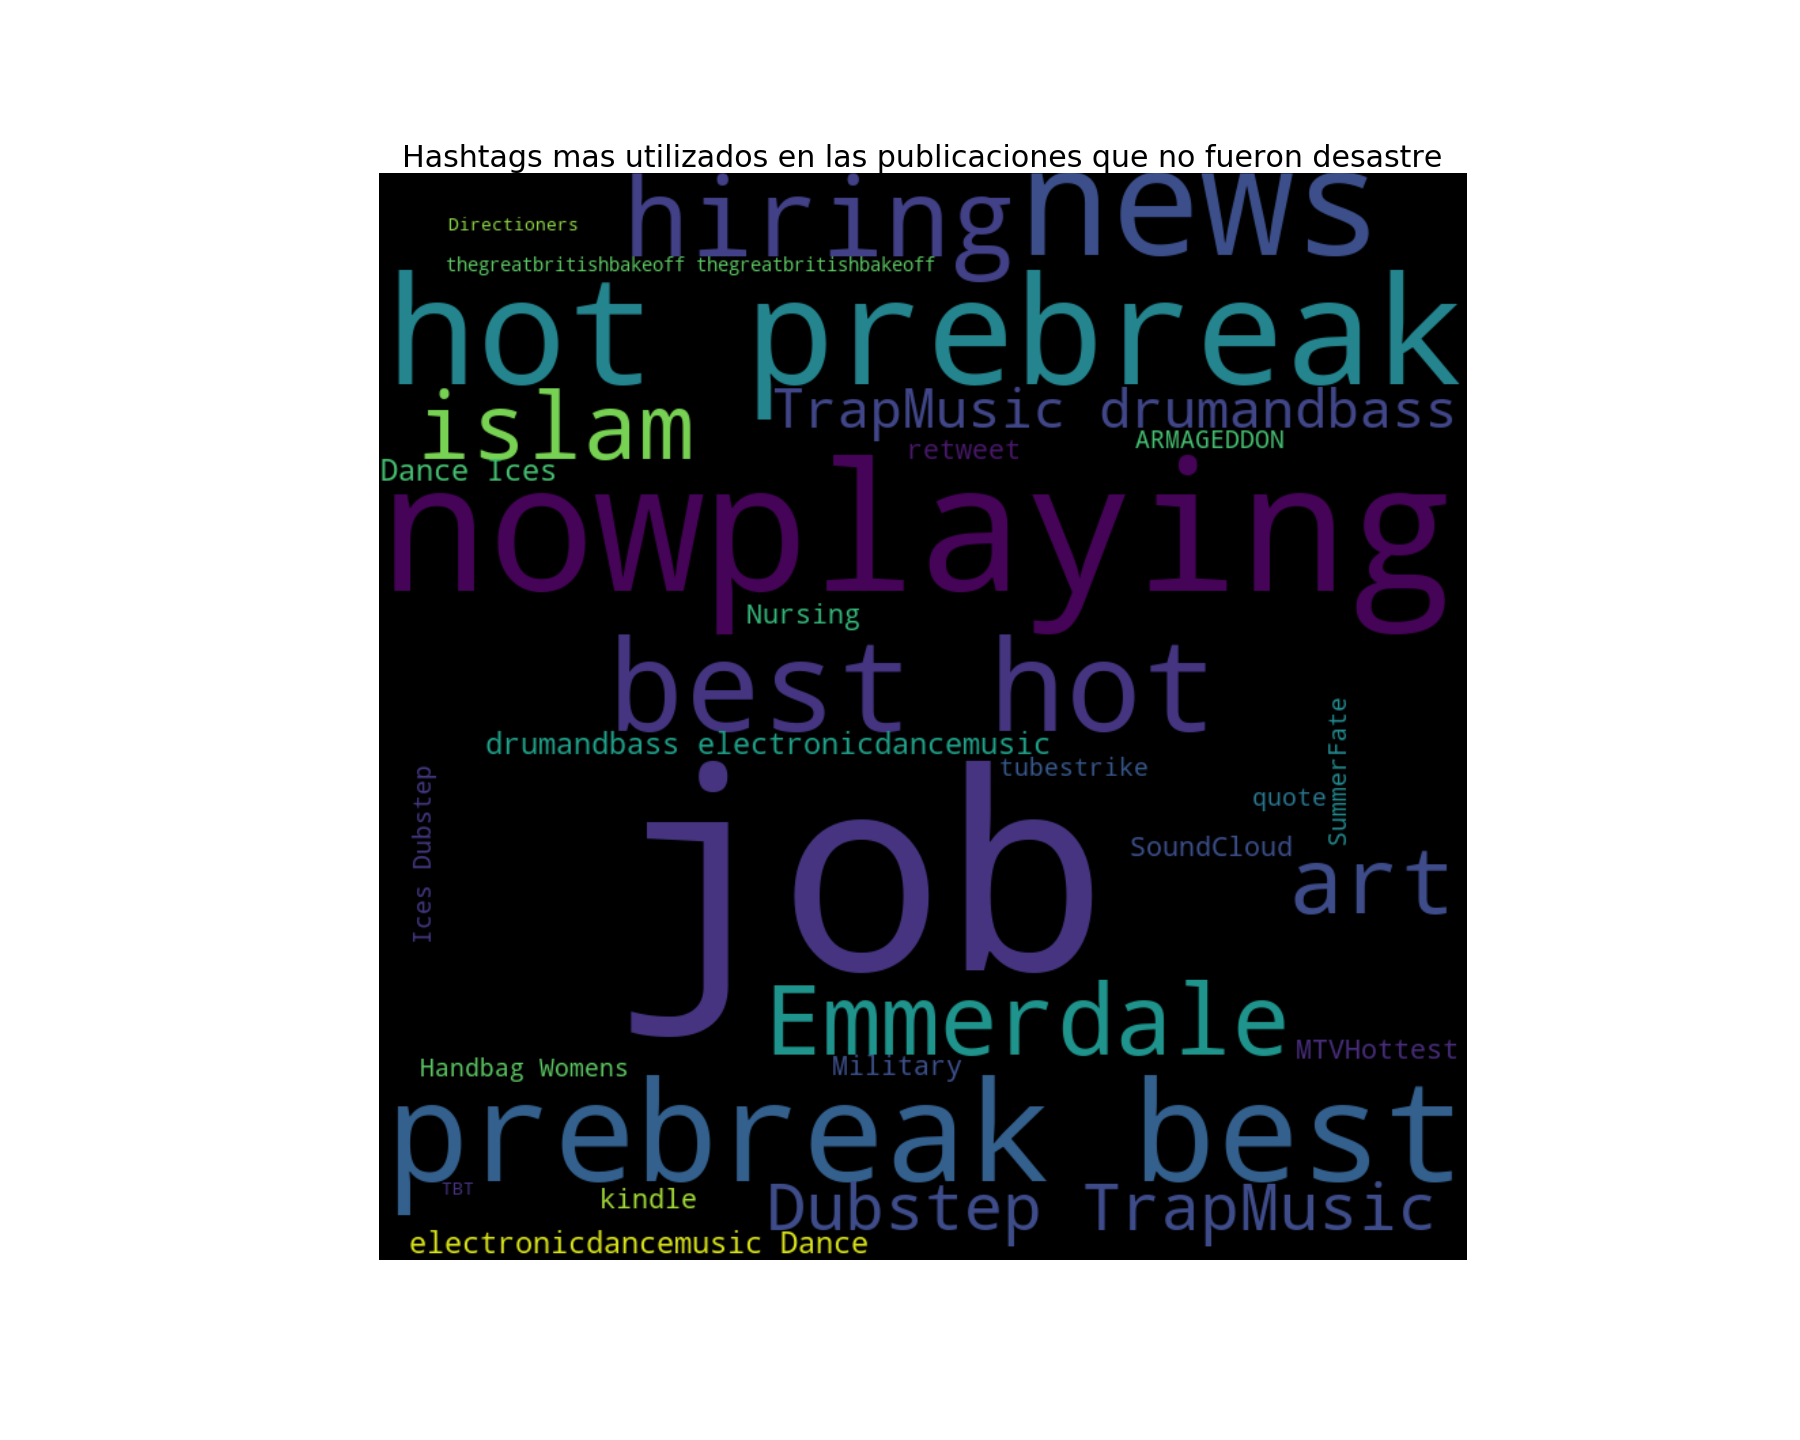
\includegraphics[width=0.85\textwidth, height=0.85\textheight, keepaspectratio]{graficos/analisis_hashtags_2.png}
\end{figure}
\begin{itemize}
    \item Vemos que es los tweets que no fueron desastres hablan la mayoría de musica.
    \item En los tweets que fueron desastre hablan sobre Hiroshima,Japón seguro son publicaciones recordando aquellos hechos.
    \item Lo que es raro es que en tweets desastre o no están presentes hashtag como hot,prebreak,best.
\end{itemize}
\par}
\subsection{\Large Distribución de la cantidad de palabras en los tweets }
{\Large
\begin{figure}[H]
 \centering
 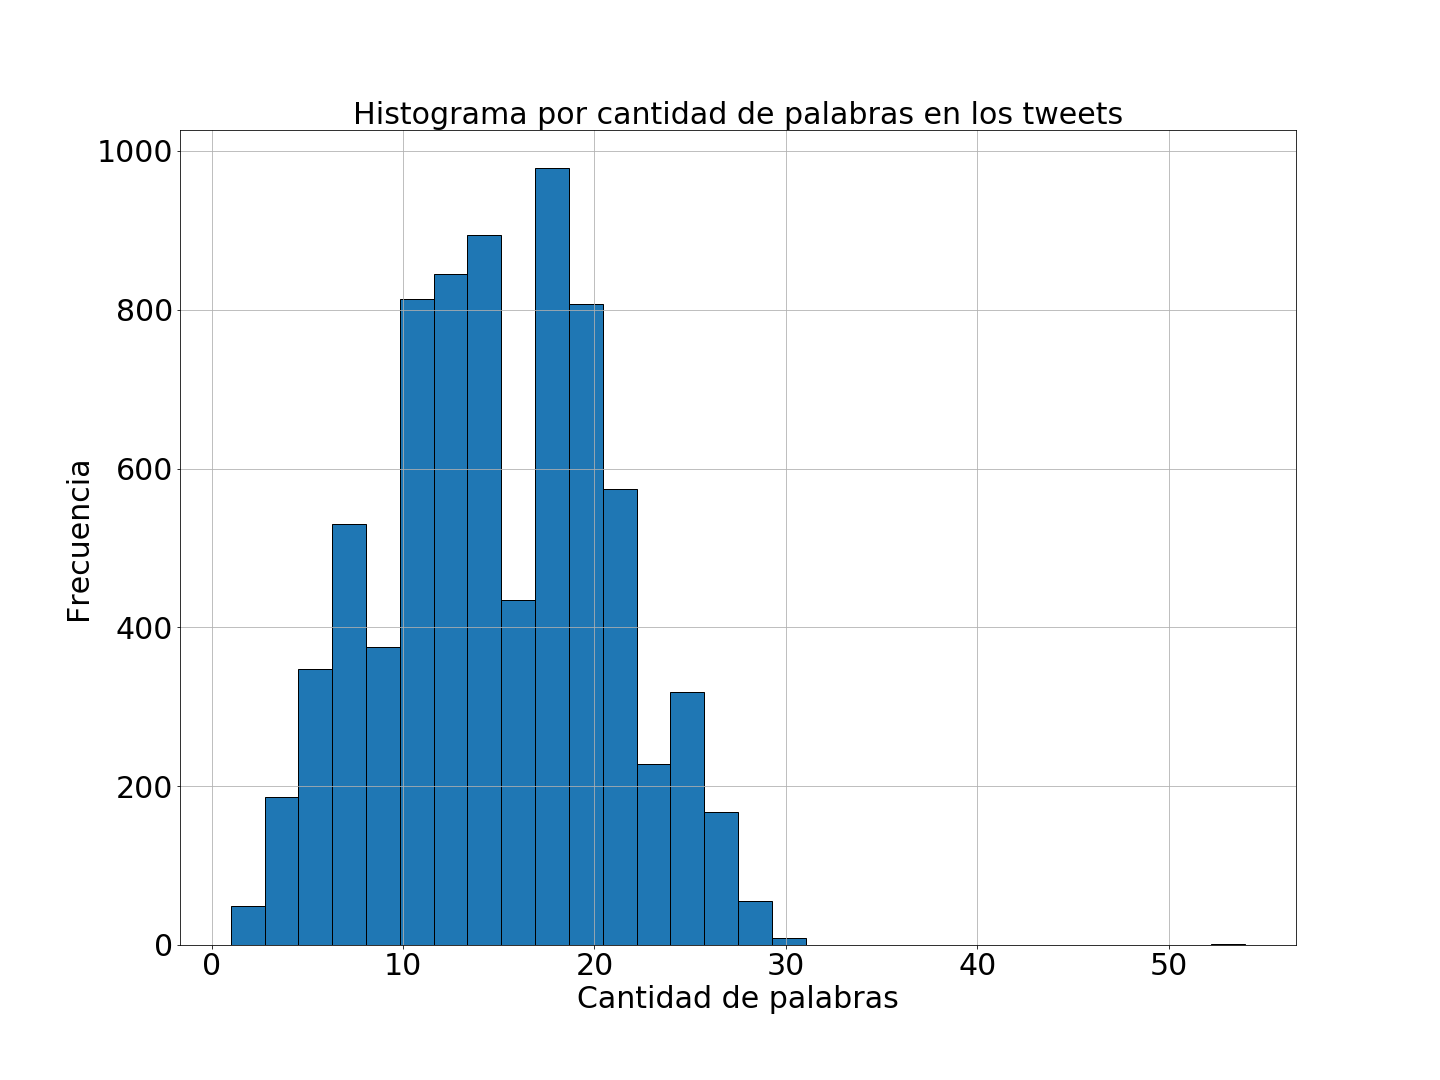
\includegraphics[width=0.8\textwidth, height=0.8\textheight, keepaspectratio]{graficos/histograma_palabras_tweets_0.png}
\end{figure}
\begin{figure}[H]
 \centering
 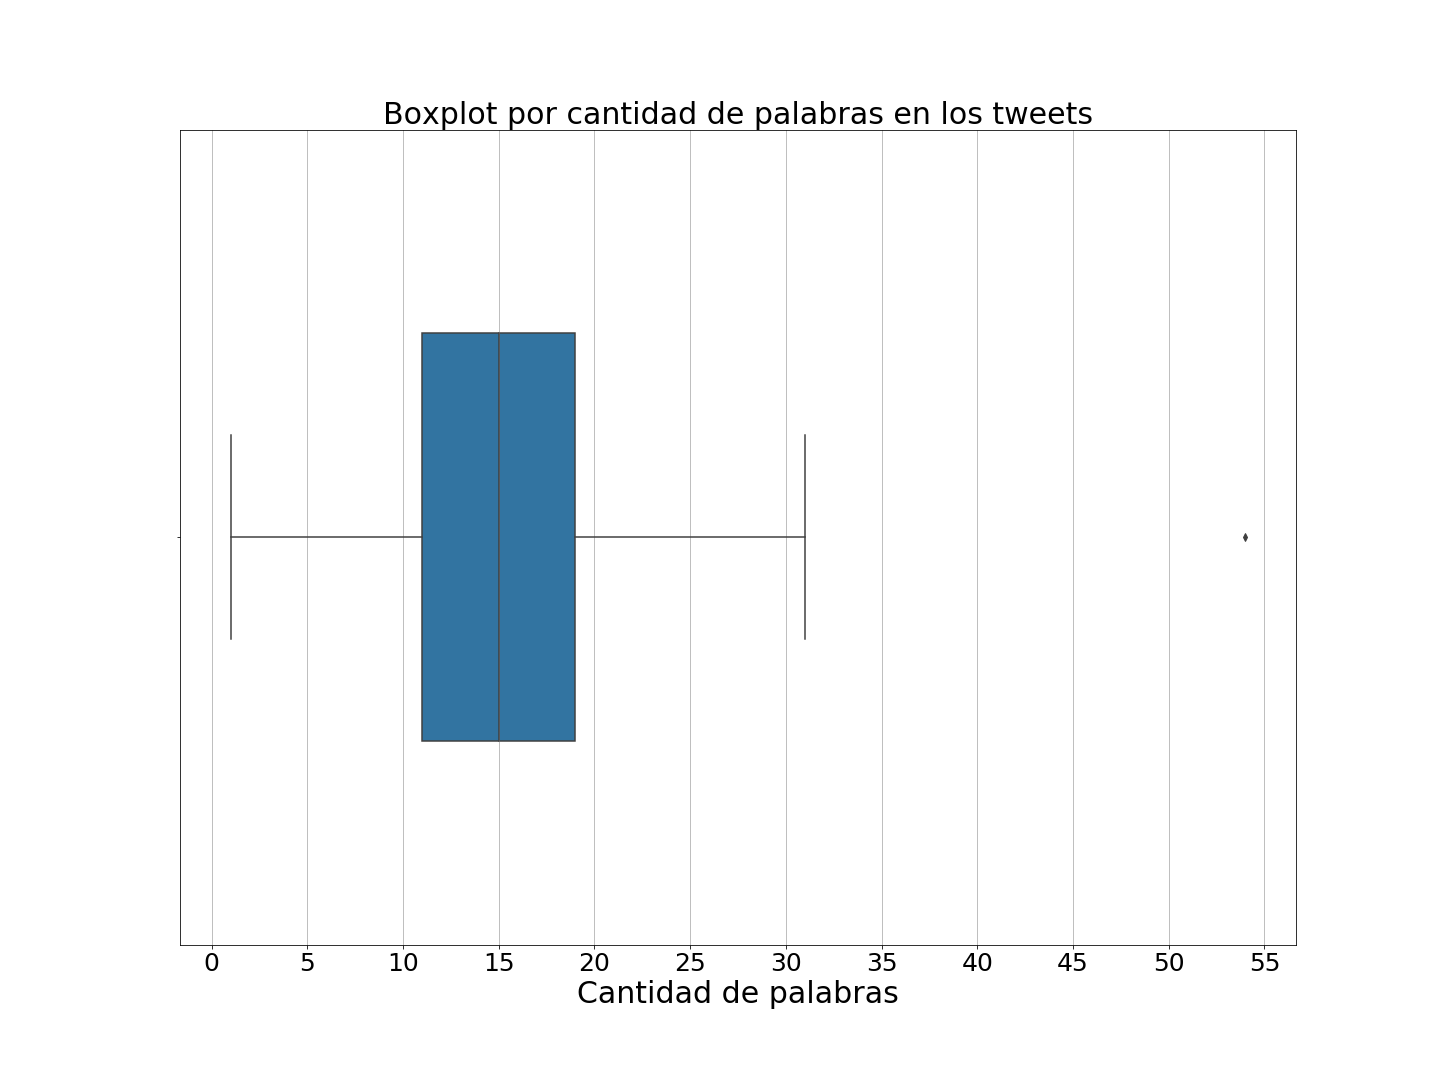
\includegraphics[width=0.8\textwidth, height=0.8\textheight, keepaspectratio]{graficos/histograma_palabras_tweets_1.png}
\end{figure}
La cantidad media de palabras utilizadas en los tweets es de 15 observando el segundo gráfico (Boxplot) vemos como tenemos un dato nada común alguien publico un tweet con mas de 50 palabras.
\begin{figure}[H]
 \centering
 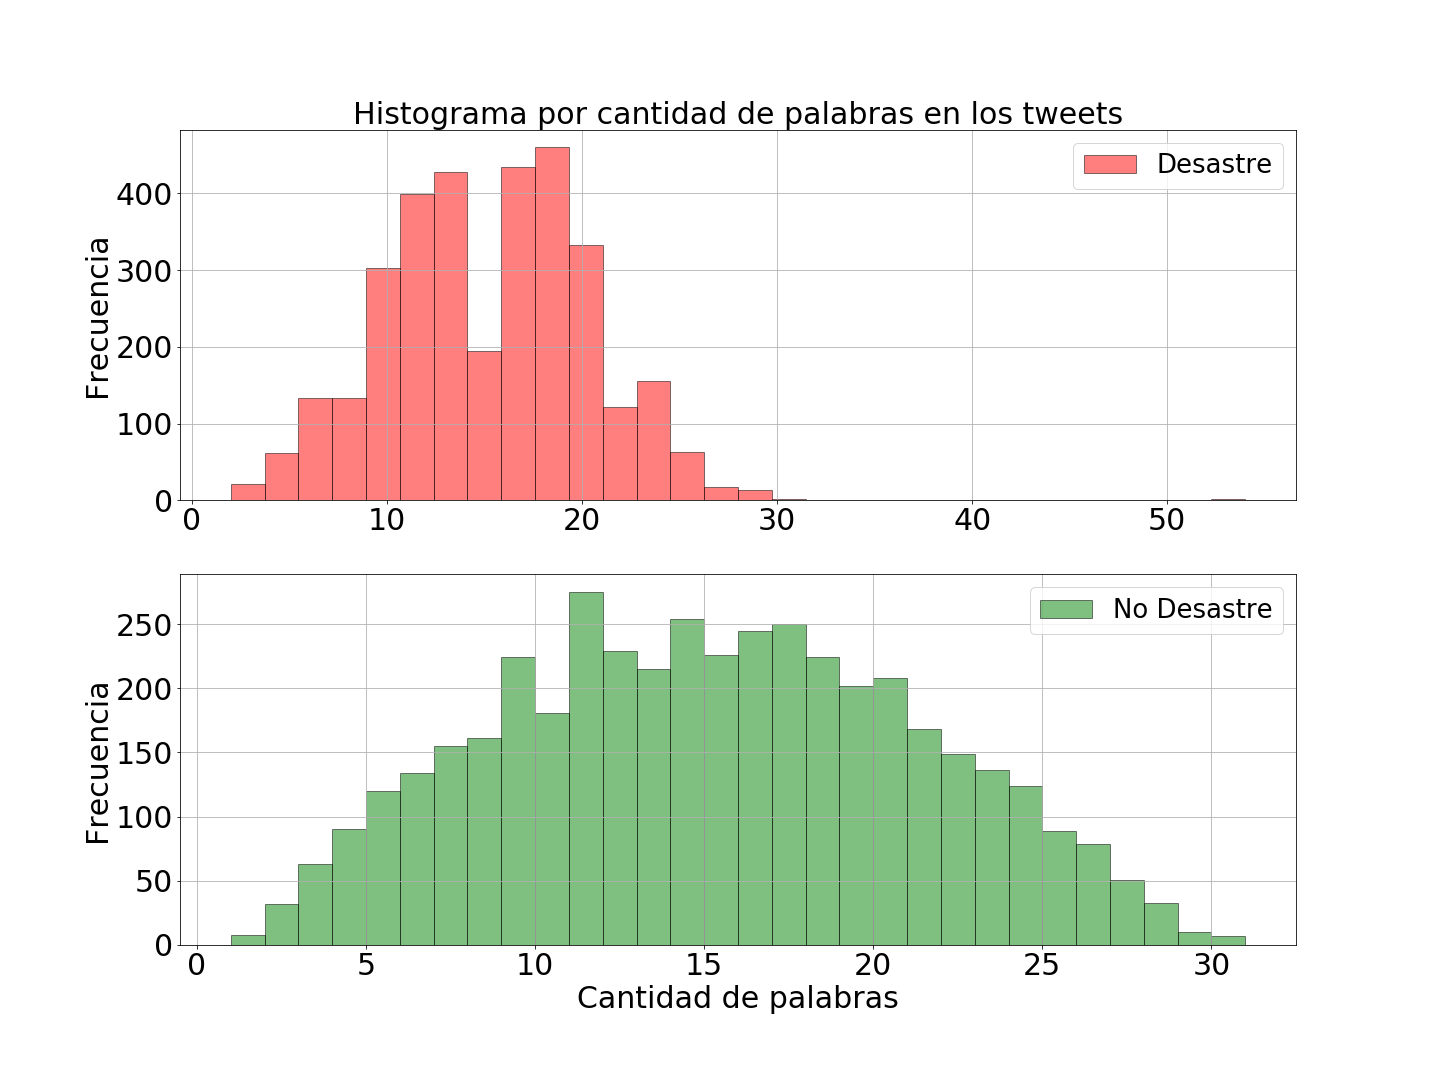
\includegraphics[width=0.8\textwidth, height=0.8\textheight, keepaspectratio]{graficos/histograma_palabras_tweets_2.png}
\end{figure}
\begin{figure}[H]
 \centering
 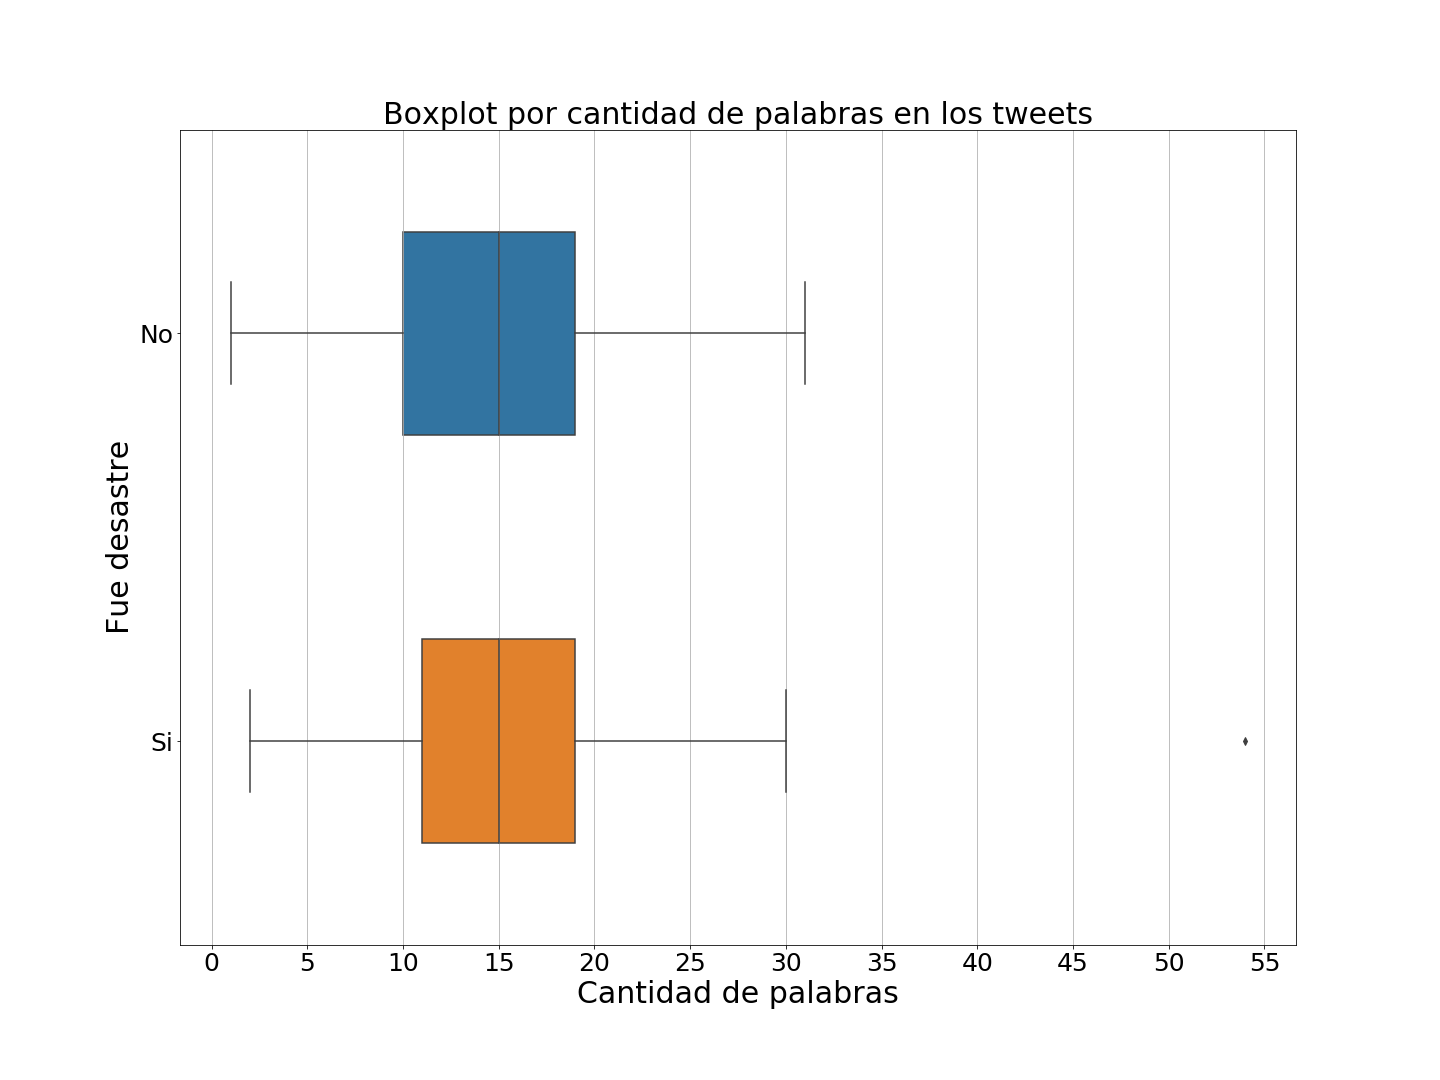
\includegraphics[width=0.8\textwidth, height=0.8\textheight, keepaspectratio]{graficos/histograma_palabras_tweets_3.png}
\end{figure}
Separando los datos tenemos, para los tweets que no son desastre una forma normal y para los tweets que son desastre podemos verlo como 2 normales solapadas entonces tenemos 2 grupos de personas los que publican tweets con mas de 15 palabras y otras con menos de 15 palabras.   
\par}
\subsection{\Large Relación del largo de la palabra y la cantidad de palabras en el texto}
{\Large
\begin{figure}[H]
 \centering
 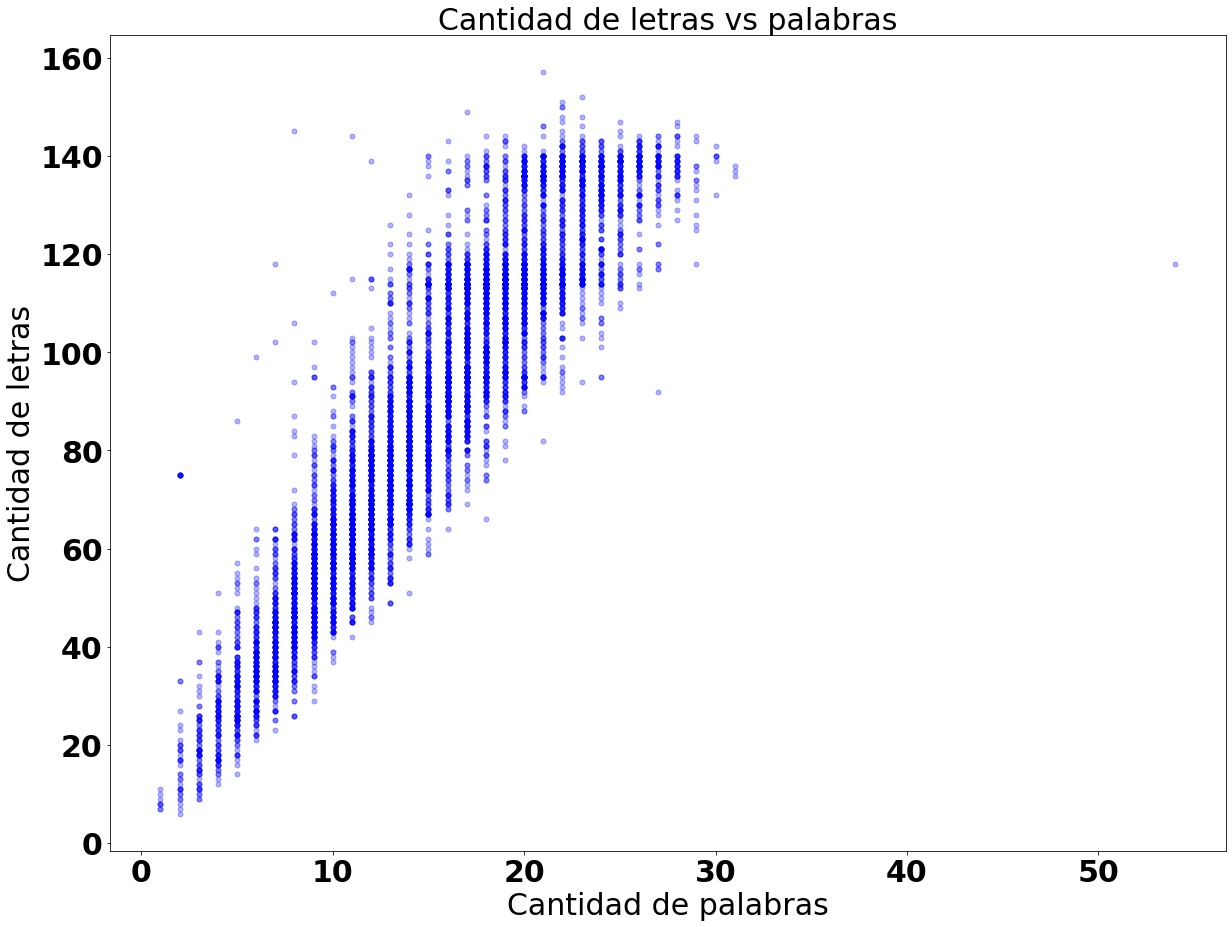
\includegraphics[width=0.8\textwidth, height=0.8\textheight, keepaspectratio]{graficos/cantidad_letras_palabras_0.png}
\end{figure}
\begin{figure}[H]
 \centering
 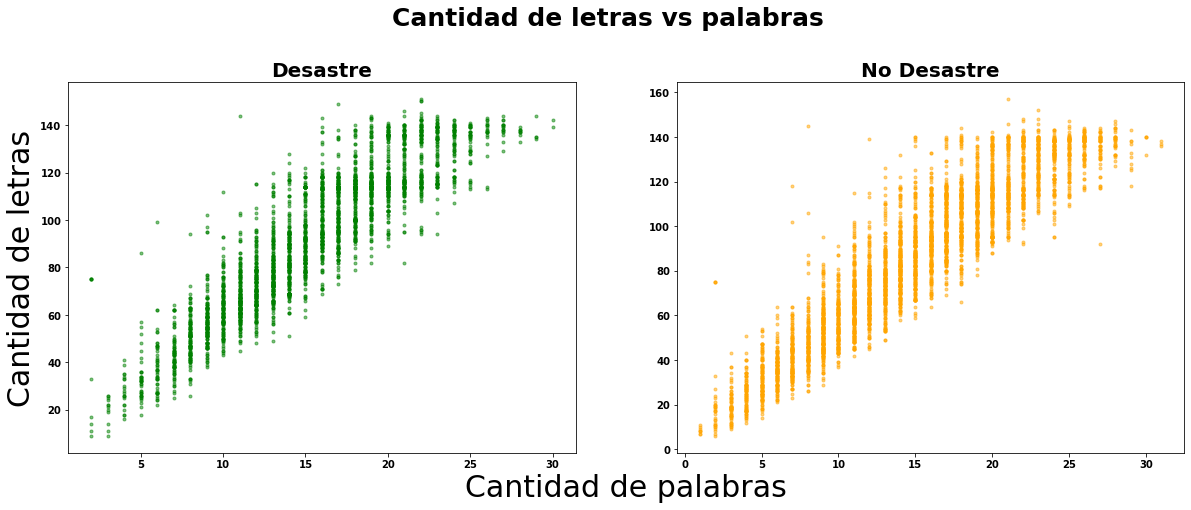
\includegraphics[width=1.1\textwidth, height=2\textheight, keepaspectratio]{graficos/cantidad_letras_palabras_1.png}
\end{figure}
\par}
\subsection{\Large Las palabras mas populares en los textos}
{\Large
\begin{figure}[H]
 \centering
 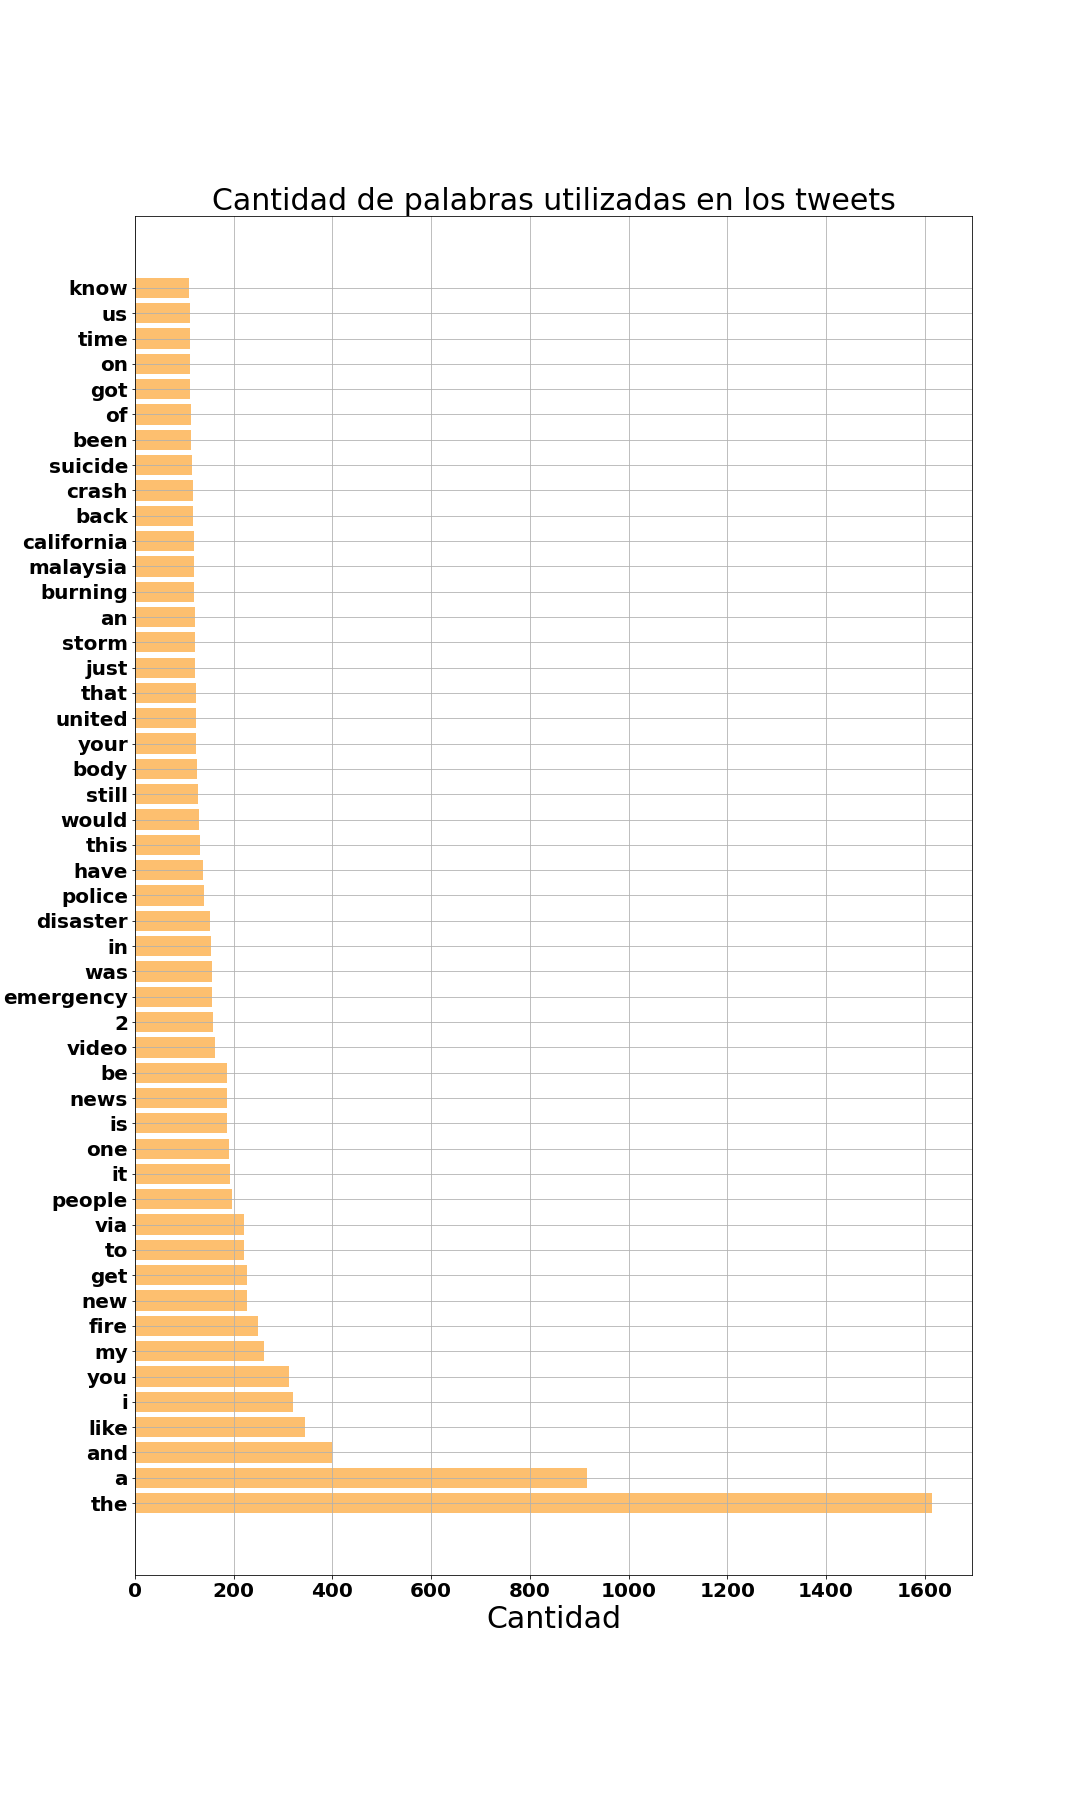
\includegraphics[width=0.8\textwidth, height=0.9\textheight, keepaspectratio]{graficos/cantidad_palabras_utilizadas_tweets_0.png}
\end{figure}
\par}
\subsection{\Large Comparación palabras mas populares en los tweets}
{\Large 
La idea es poder ver si las palabras mas populares en los tweets verdaderos y falsos tienen alguna relación con la veracidad de los mismos
\par}
{\Large
\begin{figure}[H]
 \centering
 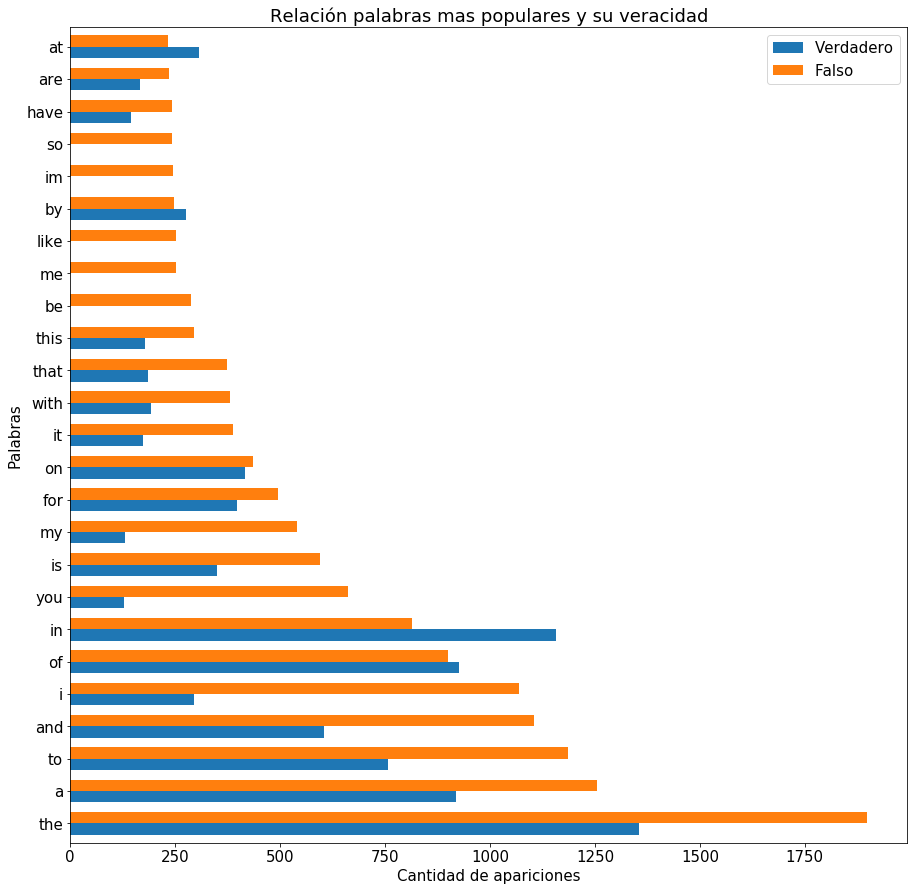
\includegraphics[width=0.8\textwidth, height=0.9\textheight, keepaspectratio]{graficos/comparacionpalabrasmaspopulares.png}
\end{figure}
{\Large 
Se puede ver que entre las palabras mas populares de los tweets verdaderos y falsos, solo las palabras "be, me, like, im, so" solo están entre las palabras mas populares de los tweets falsos, y no entre las palabras mas populares de los tweets verdaderos. Sin embargo que estas palabras no estén entre las más populares de los tweets verdaderos no significa que no estén en los tweets verdaderos. Además no son palabras para nada significativas a la hora de identificar si un tweet es verdadero o falso.
\par}
\par}
\subsection{\Large Porcentaje de tuits que tienen links}
{\Large 
La idea es poder saber si se acostumbra a poner links en los tuits, en ese caso, analizar los sitios a los que se suele apuntar y determinar posteriormente si tiene alguna relación entre la veracidad o falsedad de los tuits .\\
\par}
{\Large
\begin{figure}[H]
 \centering
 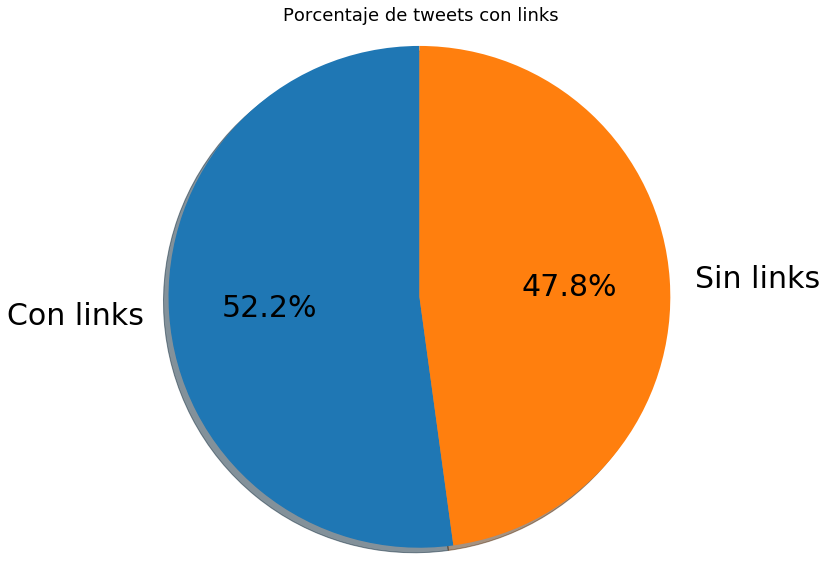
\includegraphics[width=0.8\textwidth, height=0.8\textheight, keepaspectratio]{graficos/porcentajetuitsconlinks.png}
\end{figure}
Se puede apreciar que más el porcentaje de tweets con links es alto, por lo que vale la pena analizar a donde apuntan esos links y si hay alguna relación entre la veracidad de los tweets y que tengan links o no
\par}
\subsection{\Large Relación entre los twits que tienen links y los desastres}
{\Large
\begin{figure}[H]
 \centering
 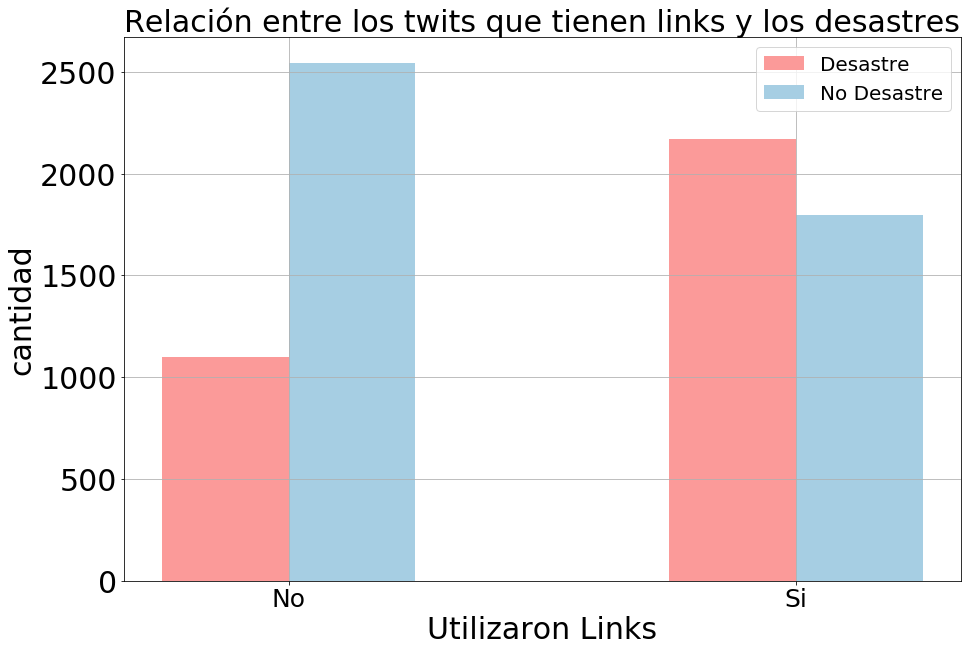
\includegraphics[width=1\textwidth, height=1\textheight, keepaspectratio]{graficos/relacion_links.png}
\end{figure}
Este gráfico muestra claramente que los twits que no tienen links tienden a ser no desastres (por mucha diferencia). En cuanto a los que tienen links tienden a ser desastres reales, pero no por tanta diferencia. Esta información resulta ser muy útil ya que si el twit no tiene links es muy probable de que no se trate de un desastre y si lo tiene, es probable de que informe acerca de un desastre.
\par}
\subsection{\Large Links mas comunes}
{\Large 
Lo que nos interesa ver es cuales son los links más comunes, para luego poder determinar si hay alguna relación por ejemplo entre tuits que tienen links a sitios de noticias y la veracidad de los mismos.\\
\par}
{\Large
\begin{figure}[H]
 \centering
 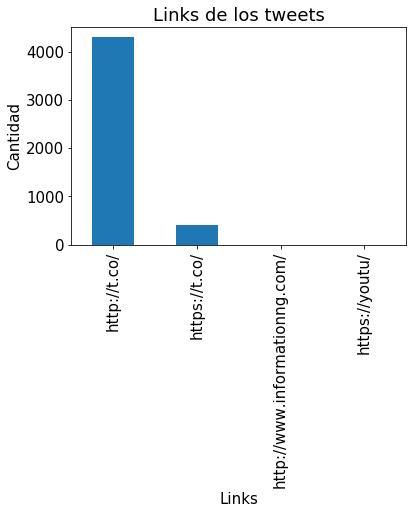
\includegraphics[width=1\textwidth, height=1\textheight, keepaspectratio]{graficos/frecuencialinks.png}
\end{figure}
Lo que podemos ver es que la mayoría de los links son acortados por twitter, por lo que no podemos saber a que sitio apuntan de forma eficiente (tendriamos que usar un API por ejemplo para averiguar a donde apuntan esos links, o hacer una petición y ver a donde redirige). 

Investigando un poco se obtiene más información de por que prácticamente todos links son acortados en este  \href{https://help.twitter.com/es/using-twitter/url-shortener}{enlace}
\par}
\subsection{\Large Relación entre los twits que tienen etiquetas y los desastres}
{\Large
\begin{figure}[H]
 \centering
 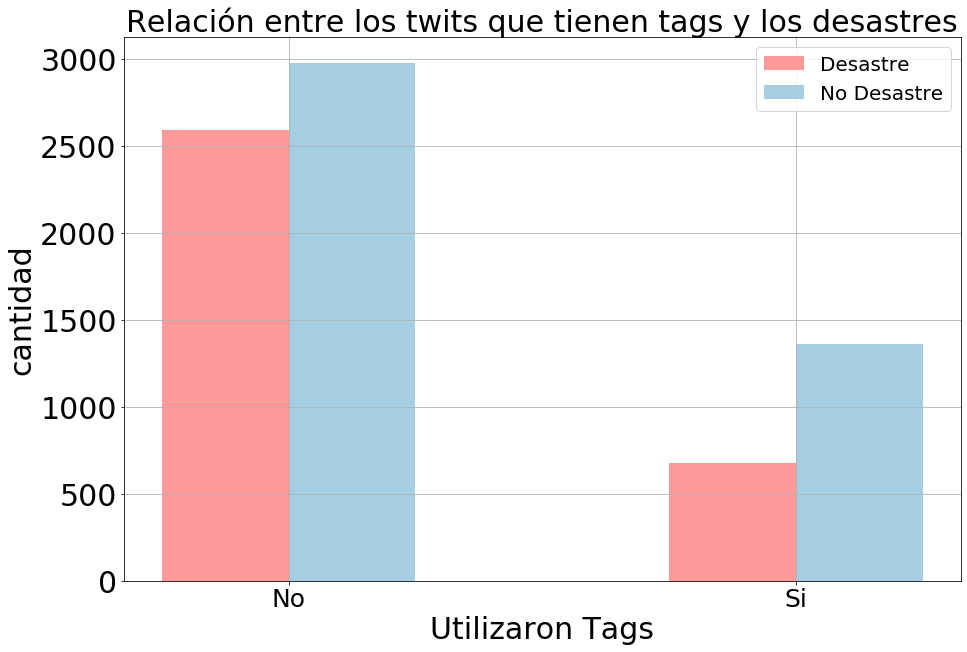
\includegraphics[width=1\textwidth, height=1\textheight, keepaspectratio]{graficos/relacion_etiquetas.png}
\end{figure}
Se puede concluir a través de este gráfico que si el tweet tiene al menos una etiqueta a otra persona, tiene bastante más chances de no ser un desastre. Si no tiene etiquetas, no se puede concluir nada ya que es muy poca la diferencia.
\par}
\section{\Large Análisis de la palabra clave}
\subsection{\Large Presencia de las Palabras Claves con los Desastres en Promedio }
{\Large
{
Dividiendo los tweets entre los que tienen o no tienen palabras claves y calculando cuántos tienen un desastre podemos comparar el porcentaje. Esto nos permite analizar si la existencia de esa categoría nos indica algo sobre la probabilidad de que el tweet se refiera a un desastre real.
\par}
\begin{figure}[H]
 \centering
 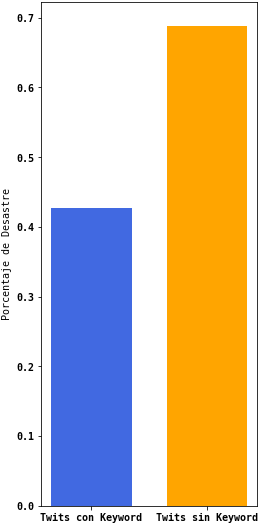
\includegraphics[width=0.7\textwidth, height=0.4\textheight, keepaspectratio]{graficos/barras_palabras_claves_desastre.png}
\end{figure}
{
Podemos ver en este gráfico como los tweets sin palabras claves tienen en promedio más desastres. Pero este dato es poco confiable debido a lo a la baja cantidad de tweets que tienen una palabra clave. 0.8\% de los tweets en nuestra base de datos no tiene una palabra clave. Por lo tanto tendríamos que no usar o usar con cuidado esta información para predecir si el tweet se refiere a un desastre real.
\par}
\begin{figure}[H]
 \centering
 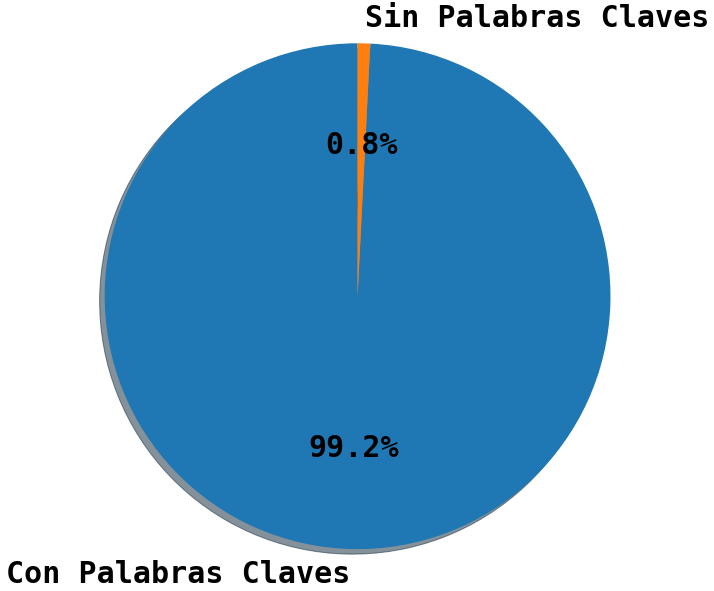
\includegraphics[width=0.5\textwidth, height=0.5\textheight, keepaspectratio]{graficos/pie_tweets_con_o_sin_palabras_claves.png}
\end{figure}
\par}
\subsection{\Large Palabras Claves con mas y menos Desastres en Total }
{\Large
Queremos saber cuales palabras aparecen mas comúnmente en el contexto de desastre, sean verdad o no. Para eso agrupamos las palabras claves de acuerdo a su raíz y hacemos un treemap de todas las palabras que aparecen por lo menos 38 veces.
\par}
{\Large
\begin{figure}[H]
 \centering
 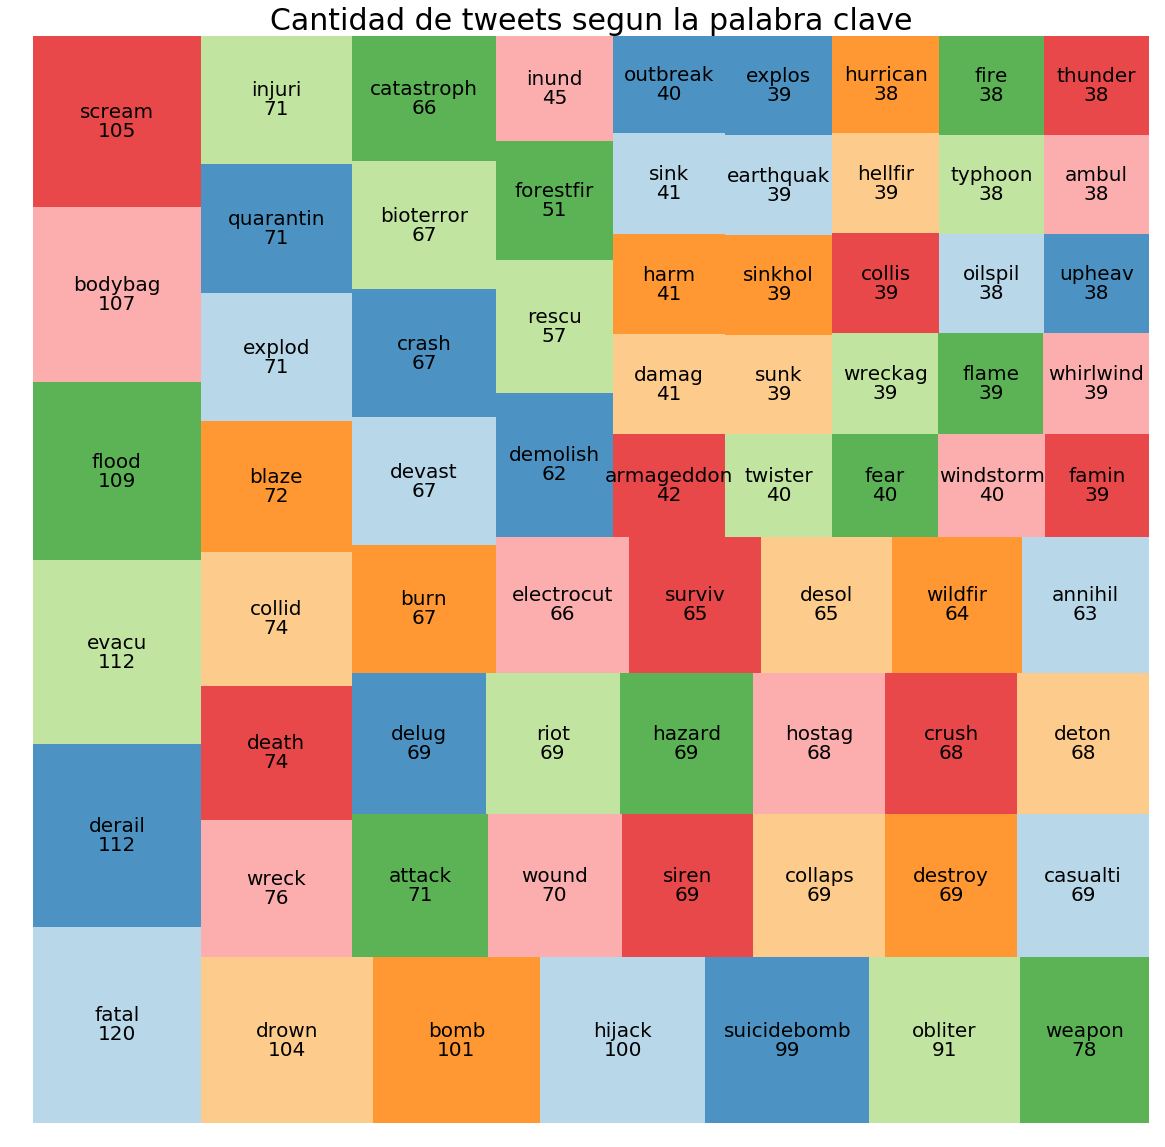
\includegraphics[width=1\textwidth, height=1\textheight, keepaspectratio]{graficos/cantidad_tweets_palabra_clave_0.png}
\end{figure}
\begin{figure}[H]
 \centering
 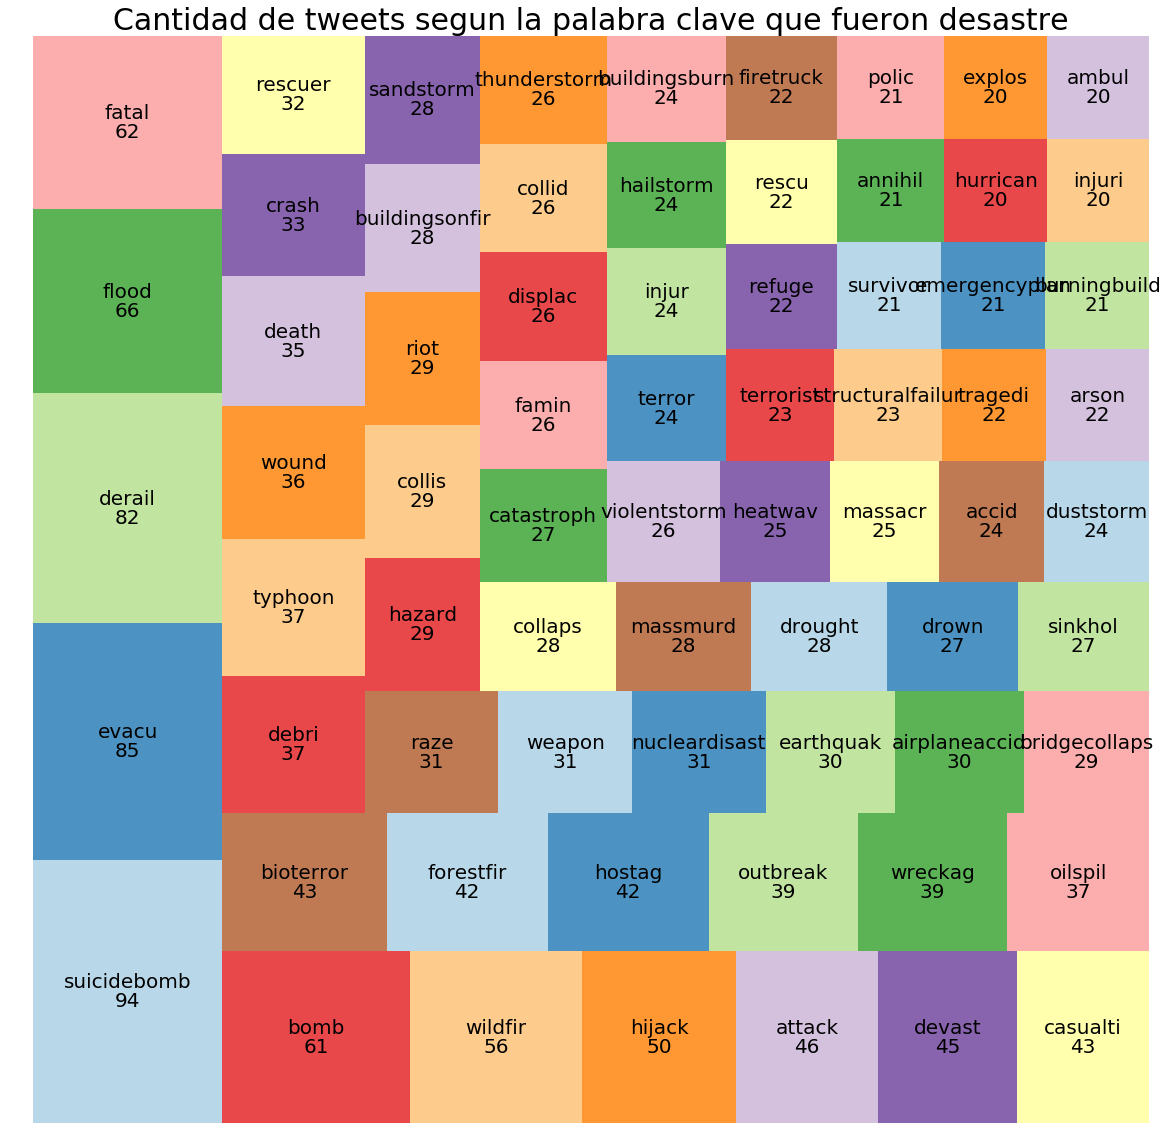
\includegraphics[width=1\textwidth, height=1\textheight, keepaspectratio]{graficos/cantidad_tweets_palabra_clave_1.png}
\end{figure}
\begin{figure}[H]
 \centering
 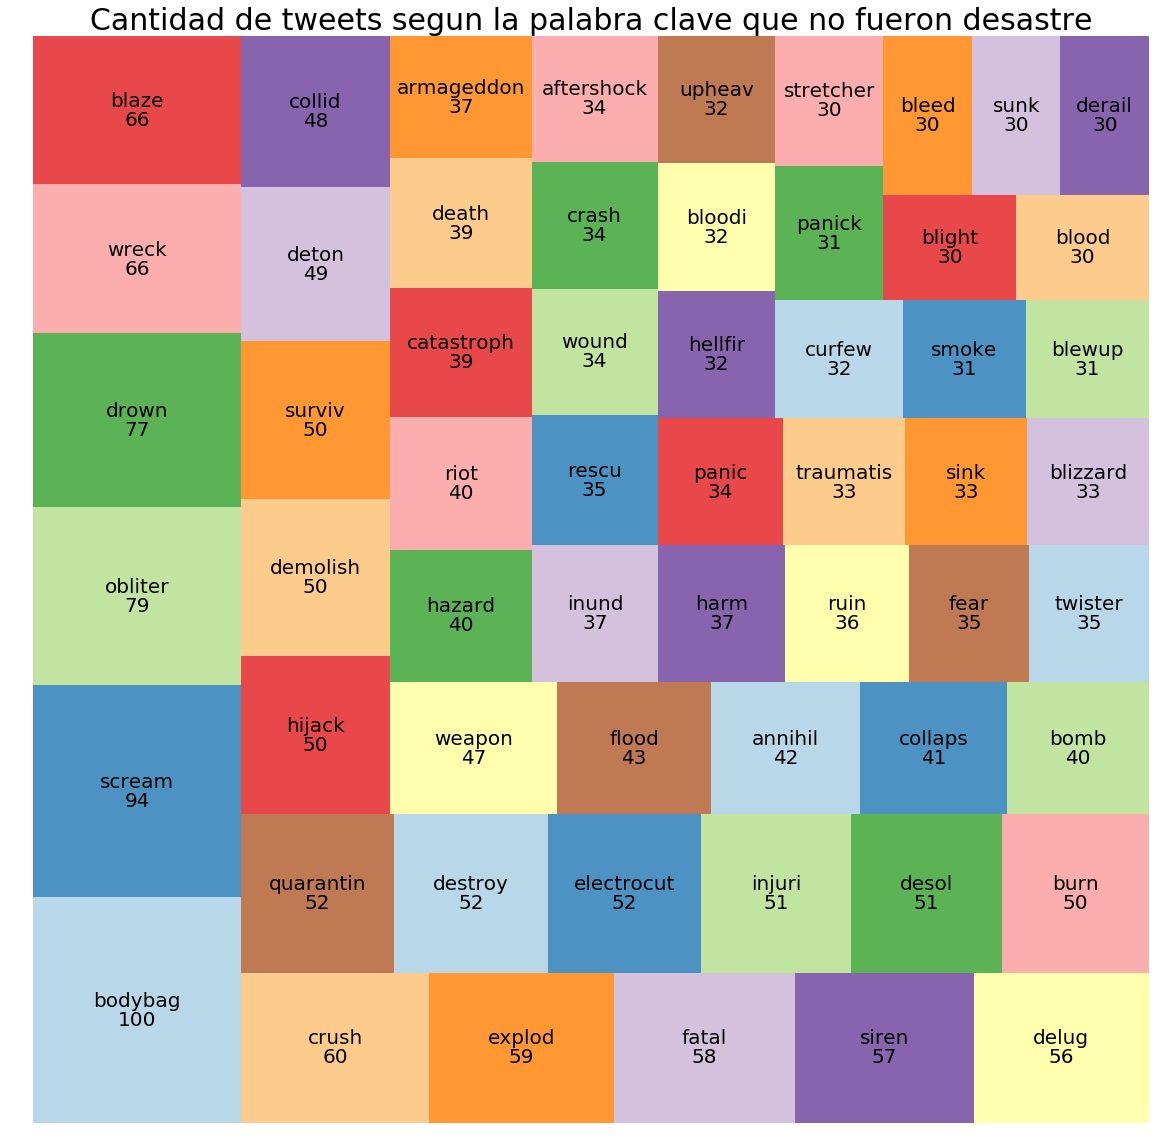
\includegraphics[width=1\textwidth, height=1\textheight, keepaspectratio]{graficos/cantidad_tweets_palabra_clave_2.png}
\end{figure}
Este gráfico nos permite ver algunas raíces mas comunes en el contexto del desastre. En particular vemos que palabras claves que empiezan con evacu- y derail- son indicadores de desastre mientras que bodybag- y scream- son ejemplos de palabras que aparecen mucho mas en casos donde no era un desastre.
\par}
\subsection{\Large Palabras Claves con mas y menos Desastres en Promedio }
{\Large
Para analizar cuales palabras claves tienen mayor porcentaje de desastres reales agrupando la base de datos y promediando los desastre. Con esto sacamos tablas de las palabras claves que tienen mayor y menor porcentaje de desastre que ocurrieron realmente. Además, agrego una columna con la muestra, para verificar que no sea un punto con muestra demasiada bajo.
\begin{figure}[H]
 \centering
 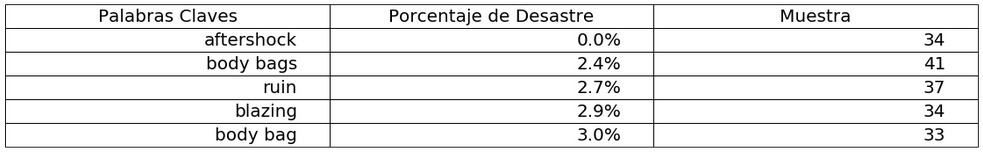
\includegraphics[width=1\textwidth, height=1\textheight, keepaspectratio]{graficos/tabla_palabras_claves_veracidad_min.png}
\end{figure}
\begin{figure}[H]
 \centering
 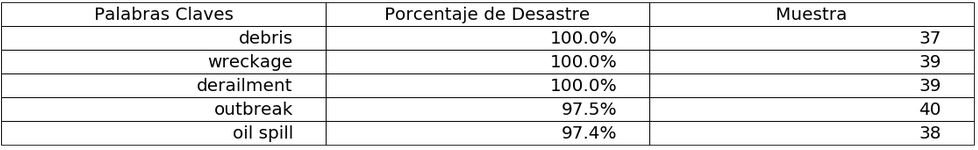
\includegraphics[width=1\textwidth, height=1\textheight, keepaspectratio]{graficos/tabla_palabras_claves_veracidad_max.png}
\end{figure}
Podemos ver que palabras como 'body bag' y 'afterschock' son usados rara vez en casos de desastres real. Mientras tant palabras como 'debris' 'wreckage' y 'oil spill' tienden a referirse a desastres reales. Este tipo de palabras nos da un indicio de que deberíamos investigar si el nivel técnico de las palabras tiene una  correlación con la probabilidad de que el desastre haya ocurrido.
\par}
\subsection{\Large Cantidad de tweets donde la palabra clave coincide con los hashtags utilizados}
{\Large
\begin{figure}[H]
 \centering
 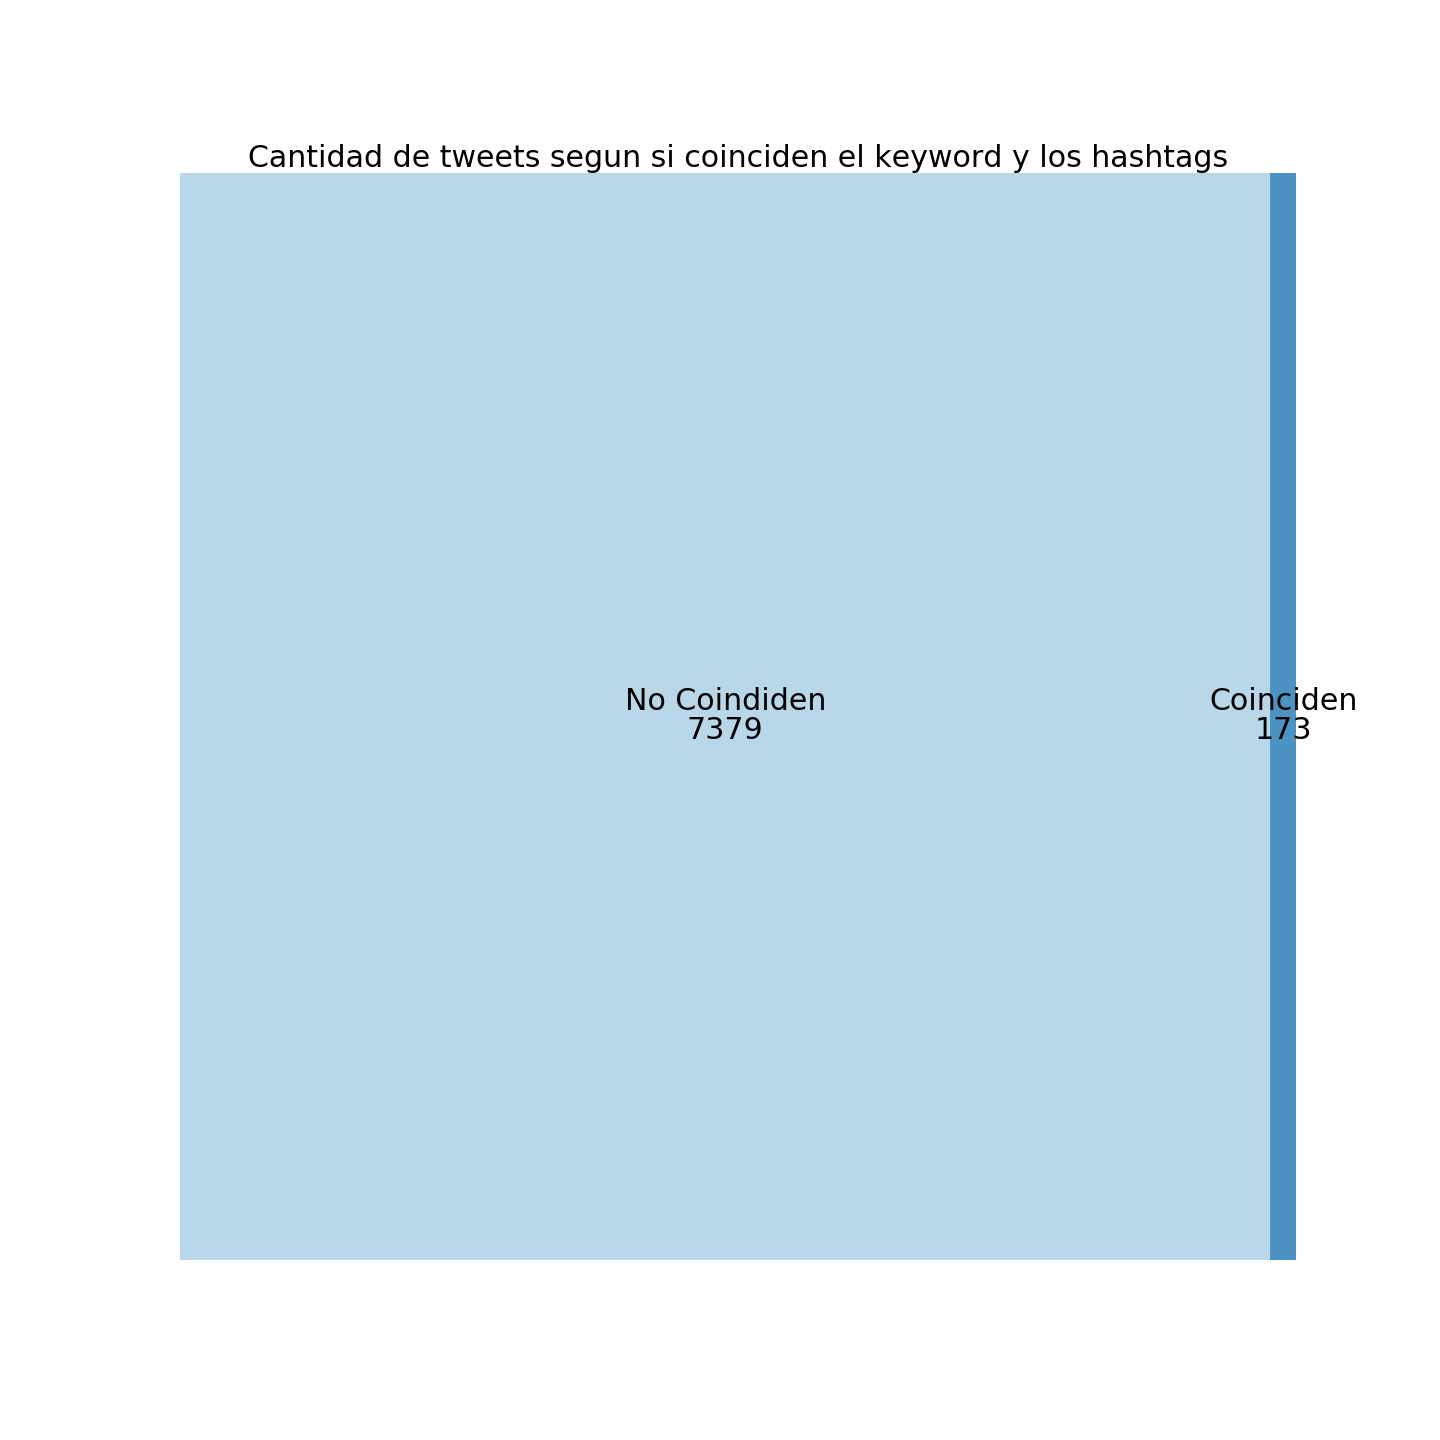
\includegraphics[width=0.8\textwidth, height=0.8\textheight, keepaspectratio]{graficos/Cantidad_tweets_keyword_hashtags_0.png}
\end{figure}
\begin{figure}[H] 
    \centering
    \subfloat{%
        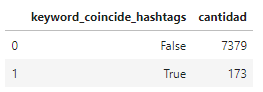
\includegraphics[width=0.5\linewidth]{graficos/Cantidad_tweets_keyword_hashtags_1.png}%
        }%
    \hfill%
    \subfloat{%
        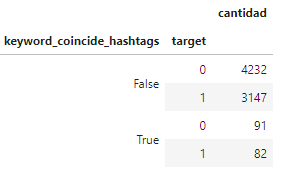
\includegraphics[width=0.5\linewidth]{graficos/Cantidad_tweets_keyword_hashtags_2.png}%
        }%
\end{figure}
Vemos que la mayoría de los hashtags utilizados no coinciden con la palabra clave,entonces con los hashtags no podemos sacar información sobre el tipo de desastre.
\par}
\section{\Large Análisis de la ubicación}
\subsection{\Large Cantidad de tweets según el lugar donde se envían}
{\Large
\begin{figure}[H]
 \centering
 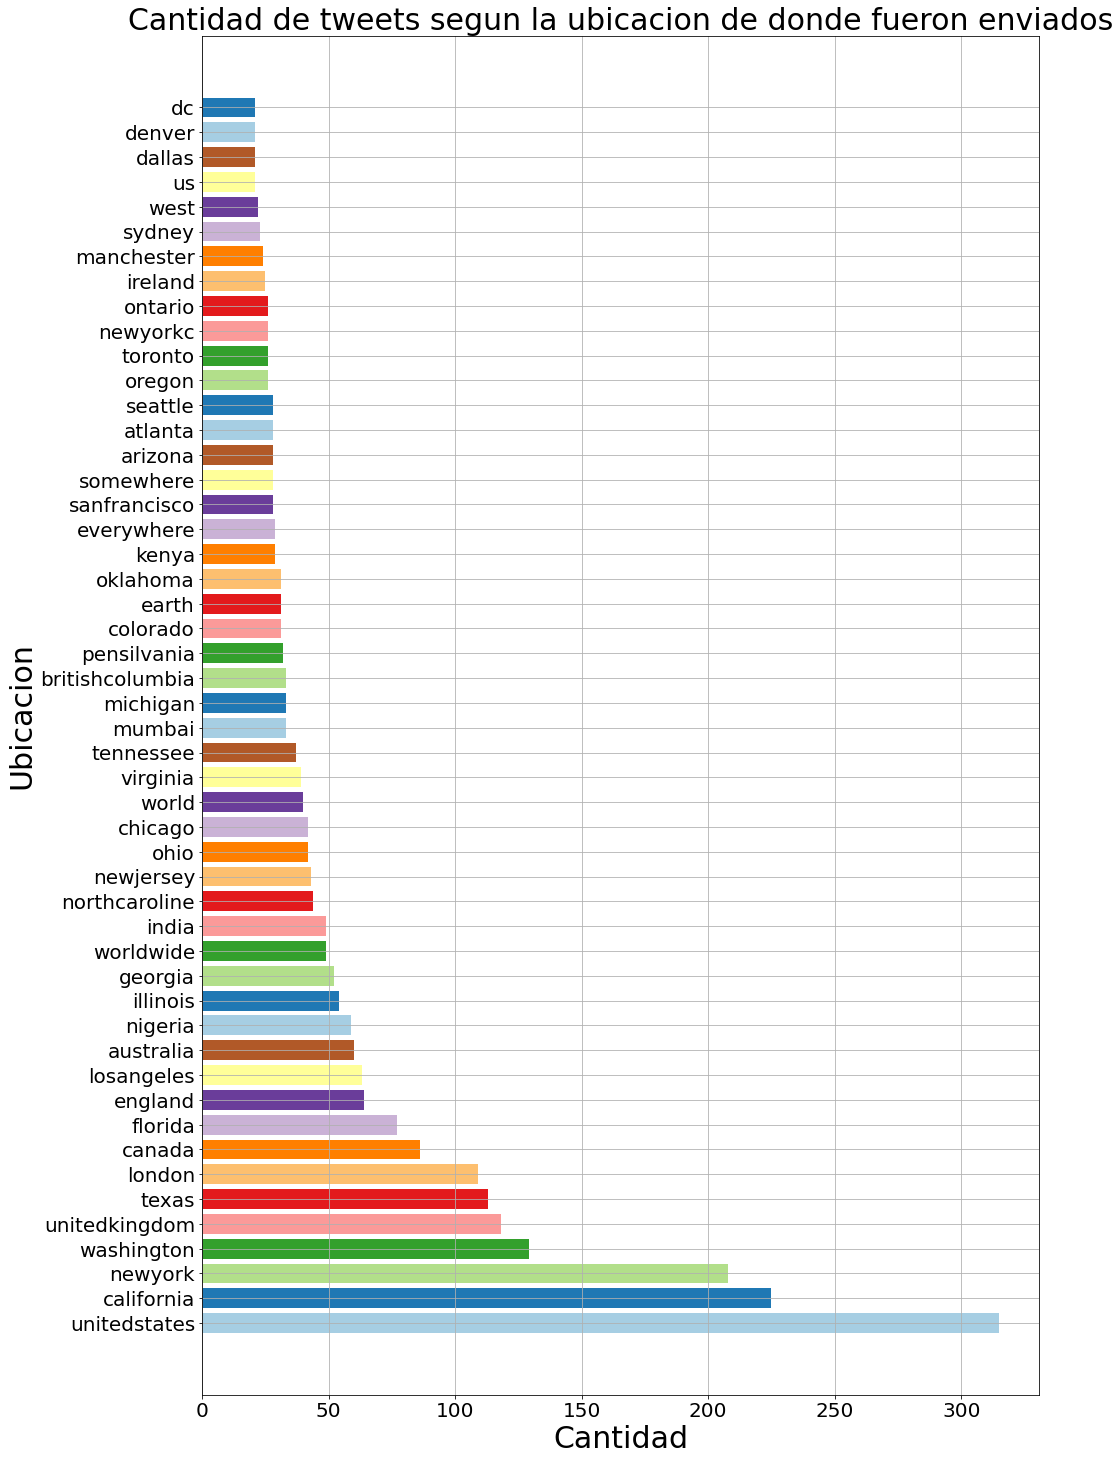
\includegraphics[width=0.8\textwidth, height=0.8\textheight, keepaspectratio]{graficos/cantidad_de_tweets_segun_la_ubicacion_0.png}
\end{figure}
\par}
\subsection{\Large Relación entre los twits que tienen localización y los desastres}
{\Large
\begin{figure}[H]
 \centering
 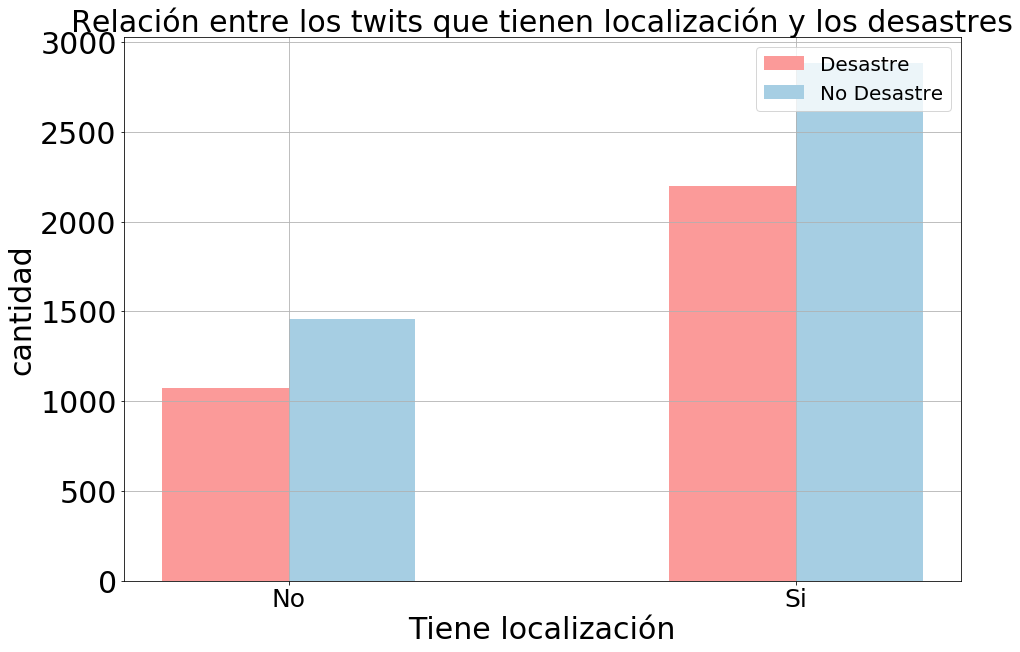
\includegraphics[width=0.8\textwidth, height=0.8\textheight, keepaspectratio]{graficos/relacion_localizacion.png}
\end{figure}
Esta visualización muestra que la relación entre los twits con o sin localización y los desastres no están para nada vinculados.
\par}
\newpage
\section{\Large Conclusiones}
\begin{itemize}
  \item Realmente no se ve relación sustancial entre la longitud de los tweets y su veracidad.
  \item En el set de datos hay tweets en varios idiomas, pero más del 96\% de los mismos están en inglés.
  \item La cantidad de tweets que no utilizan hashtags es el triple de la cantidad de tweets que usan hashtags. 
  \item En los tweets que no utilizan hashtags, hay una diferencia sustancial entre los que son veraces y los que no.
  \item En los tweets que fueron desastre los hashtags mas populares son: Japan, Hiroshima, Sismo, wildfird, WorldNews.
  \item La cantidad de palabras de los tweets se concentra alrededor de 15 palabras, a medida que usan menos palabras, o mas palabras, hay menos tweets. Sin embargo tiene un compartimiento atípico, porque para los tweets con una cantidad de palabras cercanos a la media (15 palabras) hay un decremento fuerte de tweets (se puede observar en la visualización). 
  \item Las palabras mas populares de los textos son banales: "the, a, and, like, I, you, my...".
  \item Comparando las palabras mas populares de los tweets verdaderos y falsos podemos ver que en los tweets falsos hay algunas palabras que son más populares que en los tweets falsos "be, me, like, im, so" pero es dificil explicar el por qué de esto.
  \item La cantidad de tweets que tienen links y las que no tienen es prácticamente la misma.
  \item Los links que aparecen en los tweets son en su mayoría acortados por tweeter, lo que hace dificil poder ver si hay alguna relación entre los links apuntados y la veracidad de los tweets.
  \item Las keywords que más identifican a los tweets que representan un desastre son: "fatal, flood, derail, evacu, suicidebomb, bomb, bioterror".
  \item Las ubicaciones mas comunes en los tweets son "nitedstated, california, newwork, washington, edkingdom, texas, london, canada, florida, england, losangeles, australia, nigeria".
  \item Que un link tenga localización o no, no parece estar relacionado con si representa un desastre o no.
\end{itemize}

\end{document}
